\documentclass{beamer}
\usetheme{CambridgeUS}
%%%%%%%%%%%%%%%%%%%%%%%%%%%%%%%%%%%%%%%%%%%%%%%%%%%%%%%
\setbeamercolor{block title}{bg=red!80!black, fg=white}
\setbeamercolor{block body}{bg=red!10, fg=black}
%%%%%%%%%%%%%%%%%%%%%%%%%%%%%%%%%%%%%%%%%%%%%%%%%%%%%%%
\usepackage[utf8]{vietnam}
\usepackage{tikz}
\usepackage{hyperref}
\usepackage{graphicx}
\usepackage{lipsum}
\usepackage{bookmark}
\usepackage{amsmath}
\usepackage{amssymb}

%%%%%%%%%%%%%%%%%%%%%%%%%%%%%%%%%%%%%%%%%%%%%%%%%%%%%%%
% Định nghĩa cách đánh số công thức bao gồm số chương
\numberwithin{equation}{section}
\AtBeginSection[]{
\setcounter{section}{\thesection}
\refstepcounter{section}
}
%%%%%%%%%%%%%%%%%%%%%%%%%%%%%%%%%%%%%%%%%%%%%%%%%%%%%%%
\AtBeginSection[]
{
\begin{frame}<beamer>
\frametitle{Nội dung}

\tableofcontents[
currentsection,
subsectionstyle=hide/hide,
subsubsectionstyle=hide/hide
]
\end{frame}
}
%%%%%%%%%%%%%%%%%%%%%%%%%%%%%%%%%%%%%%%%%%%%%%%%%%%%%%%
\title[{\makebox[.15\paperwidth]{MI4100 - Mật mã và độ phức tạp thuật toán}}]{Chủ đề: Mô phỏng tấn công hệ mật mã khóa công khai RSA bằng thuật toán LLL giảm lưới}
\author[Nhóm 8]{Nhóm 8}
\date[\today]{\today}
%%%%%%%%%%%%%%%%%%%%%%%%%%%%%%%%%%%%%%%%%%%%%%%%%%%%%%%
\begin{document}
%%%%%%%%%%%%%%%%%%%%%%%%%%%%%%%%%%%%%%%%%%%%%%%%%%%%%%%
% Trang tiêu đề cần có hình ảnh pictures/HUST2.jpeg
% Không chỉnh sửa gì
\begin{frame}
\begin{tikzpicture}[remember picture, overlay]
\node[anchor=center, inner sep=0pt] at (current page.center) {
\includegraphics[width=\paperwidth, height=\paperheight]{pictures/HUST2.jpeg}};
\fill[white, opacity=0.8] (current page.south west) rectangle (current page.north east);
\end{tikzpicture}
\titlepage
\end{frame}
%%%%%%%%%%%%%%%%%%%%%%%%%%%%%%%%%%%%%%%%%%%%%%%%%%%%%%%
\begin{frame}{Danh sách thành viên}
\begin{block}{Nhóm 8}
\centering
\begin{tabular} {|l|c|}
\hline
Họ và tên & MSSV \\
\hline
Nguyễn Phan Anh & 20206113 \\
Nguyễn Việt Anh & 20206115 \\
Nguyễn Đình Anh & 20206111 \\
Nguyễn Thị Hoa & 20206199 \\
Vũ Văn Nghĩa & 20206205 \\
\hline
\end{tabular}
\end{block}
\end{frame}
%%%%%%%%%%%%%%%%%%%%%%%%%%%%%%%%%%%%%%%%%%%%%%%%%%%%%%%
\begin{frame}{Phân công thành viên}
\begin{block}{Phân công thành viên}
\begin{itemize}
\item Nguyễn Phan Anh: Lập kế hoạch, phân chia công việc, phân chia công việc, xxxxxxxxxxxxxxxxxxxxxxxxxxxxxx
\item Nguyễn Việt Anh: Lập kế hoạch, phân chia công việc, phân chia công việc, xxxxxxxxxxxxxxxxxxxxxxxxxxxxxx
\item Nguyễn Đình Anh: Lập kế hoạch, phân chia công việc, phân chia công việc, xxxxxxxxxxxxxxxxxxxxxxxxxxxxxx
\item Nguyễn Thị Hoa: Lập kế hoạch, phân chia công việc, phân chia công việc, xxxxxxxxxxxxxxxxxxxxxxxxxxxxxx
\item Vũ Văn Nghĩa: Lập kế hoạch, phân chia công việc, phân chia công việc, xxxxxxxxxxxxxxxxxxxxxxxxxxxxxx
\end{itemize}
\end{block}
\end{frame}
%%%%%%%%%%%%%%%%%%%%%%%%%%%%%%%%%%%%%%%%%%%%%%%%%%%%%%%
%! %%%%%%%%%%%%%%%%%%%%%%%%%%%%%%%%%%%%%%%%%%%%%%%%%%%%%%
%! %%%%%%%%%%%%%%%%%%%%%%%%%%%%%%%%%%%%%%%%%%%%%%%%%%%%%%
%! %%%%%%%%%%%%%%%%%%%%%%%%%%%%%%%%%%%%%%%%%%%%%%%%%%%%%%
%! %%%%%%%%%%%%%%%%%%%%%%%%%%%%%%%%%%%%%%%%%%%%%%%%%%%%%%
%! %%%%%%%%%%%%%%%%%%%%%%%%%%%%%%%%%%%%%%%%%%%%%%%%%%%%%%
\section{Tổng quan về hệ mật mã khóa công khai}
\subsection{Lịch sử}
\begin{frame}{Lịch sử}

\begin{itemize}
\item Hệ mật mã khóa công khai là một bước tiến lớn và là cuộc cách mạng trong lĩnh vực mật mã
\item Hệ mật mã khóa công khai được Diffie và Hellman đưa ra năm 1976
\end{itemize}

\begin{columns}

\begin{column}{0.4\textwidth}
\begin{figure}[H]
\centering
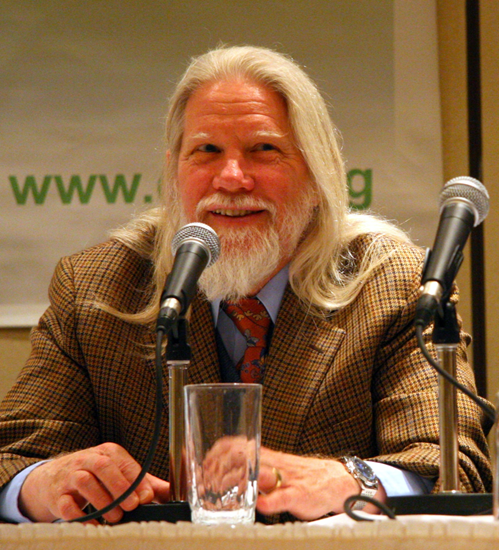
\includegraphics[scale = 0.4]{pictures/Bailey_Whitfield_Diffie.png}
\end{figure}
Bailey Whitfield 'Whit' Diffie\\ (sinh 05/06/1944 – 80 tuổi)
\end{column}

\begin{column}{0.4\textwidth}
\begin{figure}[H]
\centering
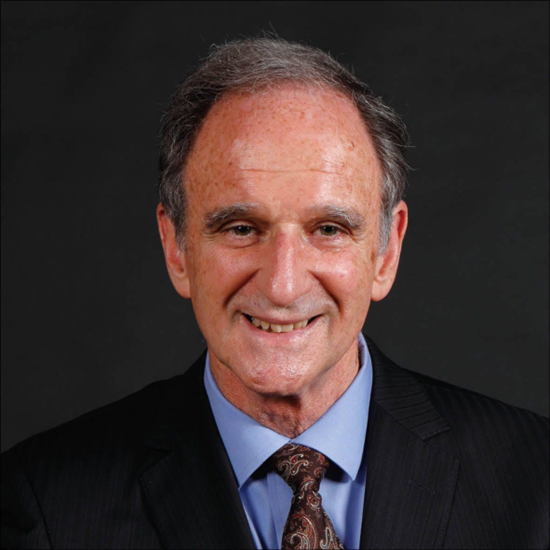
\includegraphics[scale = 0.4]{pictures/Martin_Edward_Hellman.png}
\end{figure}
Martin Edward Hellman\\(sinh 02/10/1945 - 79 tuổi)
\end{column}

\end{columns}

\end{frame}
%%%%%%%%%%%%%%%%%%%%%%%%%%%%%%%%%%%%%%%%%%%%%%%%%%%%%%%
\subsection{Khái niệm}
\begin{frame}{Khái niệm}

\begin{itemize}
\item Hệ mật mã khóa công khai là một dạng mật mã hoá cho phép người sử dụng trao đổi các thông tin mật mà không cần phải trao đổi các khoá chung bí mật trước đó
\item Việc mã hóa công khai được thực hiện bằng cách sử dụng một cặp khóa có quan hệ toán học với nhau là khóa công khai và khoá bí mật
\begin{itemize}
\item Khóa công khai: được công khai phổ biến - dùng để mã hóa
\item Khóa bí mật: được giữ bí mật - dùng để giải mã
\end{itemize}
\end{itemize}

$\Rightarrow$ Điều này đảm bảo hệ thống là không thể (hoặc rất khó) tìm ra khóa bí mật nếu chỉ biết khóa công khai

\end{frame}
%%%%%%%%%%%%%%%%%%%%%%%%%%%%%%%%%%%%%%%%%%%%%%%%%%%%%%%
\subsection{Mô hình tổng quát}
\begin{frame}{Mô hình tổng quát}
\begin{figure}[H]
\centering
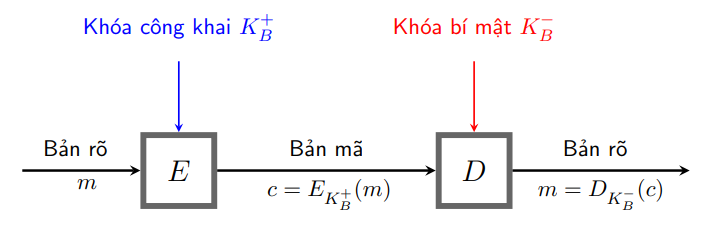
\includegraphics[scale = 0.6]{pictures/mo_hinh_tong_quat.png}
\end{figure}

\begin{block}{Nhận xét}
Hệ mật mã khóa công khai được gọi là hệ mật mã bất đối xứng vì mã hóa và giải mã sử dụng khóa khác nhau
\end{block}
\end{frame}
%%%%%%%%%%%%%%%%%%%%%%%%%%%%%%%%%%%%%%%%%%%%%%%%%%%%%%%
\subsection{Ưu, nhược điểm của hệ mã hóa công khai}
\begin{frame}{Ưu điểm}
\begin{itemize}
\item Thuật toán được viết một lần, công khai cho nhiều lần dùng, cho nhiều người dùng, họ chỉ cần giữ bí mật khóa riêng của mình
\item Khi biết các tham số ban đầu của hệ mã hóa, việc tính ra cặp khoá công khai và bí mật phải là "dễ", tức là trong thời gian đa thức
\item Khả năng lộ khóa bí mật khó hơn vì chỉ có một người giữ gìn. Nếu thám mã biết khoá công khai, cố gắng tìm khoá bí mật, thì chúng phải đương đầu với bài toán "khó"
\item Nếu thám mã biết khoá công khai và bản mã, thì việc tìm ra bản rõ cũng là bài toán "khó"
\end{itemize}
\end{frame}
%%%%%%%%%%%%%%%%%%%%%%%%%%%%%%%%%%%%%%%%%%%%%%%%%%%%%%%
\begin{frame}{Nhược điểm}
\begin{itemize}
\item Hệ mã hóa khóa công khai: mã hóa và giải mã chậm hơn hệ mã hóa khóa bí mật
\item Khả năng bị tấn công dạng tấn công người đứng giữa do kẻ tấn công lợi dụng việc phân phối khóa công khai để thay giả mạo gói tin
\end{itemize}
\end{frame}
%%%%%%%%%%%%%%%%%%%%%%%%%%%%%%%%%%%%%%%%%%%%%%%%%%%%%%%
\subsection{So sánh với mã đối xứng}
\begin{frame}{So sánh với mã đối xứng}

\end{frame}
%%%%%%%%%%%%%%%%%%%%%%%%%%%%%%%%%%%%%%%%%%%%%%%%%%%%%%%
%! %%%%%%%%%%%%%%%%%%%%%%%%%%%%%%%%%%%%%%%%%%%%%%%%%%%%%%
%! %%%%%%%%%%%%%%%%%%%%%%%%%%%%%%%%%%%%%%%%%%%%%%%%%%%%%%
%! %%%%%%%%%%%%%%%%%%%%%%%%%%%%%%%%%%%%%%%%%%%%%%%%%%%%%%
%! %%%%%%%%%%%%%%%%%%%%%%%%%%%%%%%%%%%%%%%%%%%%%%%%%%%%%%
%! %%%%%%%%%%%%%%%%%%%%%%%%%%%%%%%%%%%%%%%%%%%%%%%%%%%%%%
\section{Hệ mật mã RSA}
\subsection{Tổng quan về hệ mật mã RSA}
\begin{frame}{Tổng quan về hệ mật mã RSA}

\begin{itemize}
\item RSA là hệ mật mã khóa công khai phổ biến nhất trong thực tế, phát minh bởi Rivest, Shamir và Adleman (1977)
\item Cơ sở thuật toán RSA dựa trên tính khó của bài toán phân tích các số lớn ra thừa số nguyên tố: không tồn tại thuật toán thời gian đa thức (theo độ dài của biểu diễn nhị phân của số đó) cho bài toán này.
\end{itemize}

\begin{figure}[H]
\centering
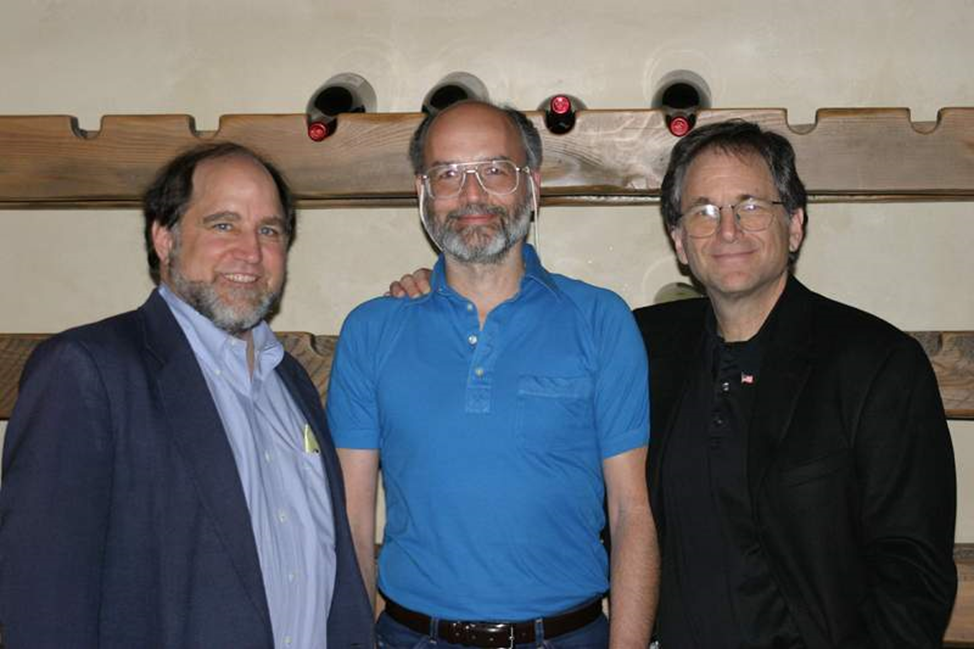
\includegraphics[scale = 0.4]{pictures/RSA_RonRivestAdiShamirLeonardAdleman.png}
\end{figure}

\end{frame}
%%%%%%%%%%%%%%%%%%%%%%%%%%%%%%%%%%%%%%%%%%%%%%%%%%%%%%%
\subsection{Bảng chữ cái RSA}
\begin{frame}{Bảng chữ cái RSA}

\end{frame}
%%%%%%%%%%%%%%%%%%%%%%%%%%%%%%%%%%%%%%%%%%%%%%%%%%%%%%%
\subsection{Mã hóa và giải mã RSA}
\begin{frame}{Mã hóa và giải mã RSA}
\begin{itemize}
\item Bảo mật của RSA dựa trên giả thuyết không có các thuật toán đủ nhanh để khai triển luỹ thừa một số. Qui trình áp dụng RSA gồm hai bước:
\begin{enumerate}
\item Lựa chọn (sinh) cặp khóa công khai và khóa bí mật
\item Thực hiện thuật toán mã hoá và thuật toán giải mã
\end{enumerate}
\end{itemize}
\end{frame}
%%%%%%%%%%%%%%%%%%%%%%%%%%%%%%%%%%%%%%%%%%%%%%%%%%%%%%%
\begin{frame}{Thuật toán sinh khóa}

\begin{enumerate}
\item Chọn hai số nguyên tố đủ lớn, $p$ và $q$
\item Tính toán $n = pq$ và $\phi(n) = (p - 1)(q - 1)$
\item Chọn một số, $e$ $(1 < e < \phi(n))$ sao cho $\text{gcd}(e, \phi(n)) = 1$.

Giá trị $e$ sẽ được sử dụng trong mã hoá
\item Tìm một số $d$ sao cho $ed - 1$ chia hết cho $\phi(n)$, hay nói cách khác $d = e^{-1} \mod \phi(n)$. Giá trị $d$ sẽ được sử dụng để giải mã
\item Công khai khóa $K^+_B$ = (n, e) và giữ bí mật khóa $K^-_B$ = (n, d)
\end{enumerate}

\end{frame}
%%%%%%%%%%%%%%%%%%%%%%%%%%%%%%%%%%%%%%%%%%%%%%%%%%%%%%%
\begin{frame}{Mã hóa và giải mã RSA}

\begin{columns}

\begin{column}{0.6\textwidth}

\begin{itemize}

\item Mã hóa:

\[
c = E (m, K_B^+) = m^e \mod n
\]

\item Giải mã:

\[
m = D (c, K_B^-) = c^d \mod n
\]

\end{itemize}

\end{column}

\begin{column}{0.4\textwidth}

\includegraphics[width=\textwidth]{pictures/chu-ky-so-rsa-1.jpg}
\end{column}

\end{columns}

\end{frame}
%%%%%%%%%%%%%%%%%%%%%%%%%%%%%%%%%%%%%%%%%%%%%%%%%%%%%%%
\begin{frame}{Ví dụ về RSA}

\begin{block}{Ví dụ}
Cho bản rõ \(M = 15 \) sử dụng thuật toán RSA với \(p = 11 \), \(q = 3 \)
\end{block}

\textbf{Thuật toán sinh khóa:}

\begin{itemize}
\item Bước 1: \textbf{Với hai số nguyên tố}:
$p = 11, \quad q = 3 \quad \Rightarrow \quad n = p \cdot q = 11 \cdot 3 = 33$
\item Bước 2: \textbf{Tính hàm Euler}:
\[
\varphi(n) = (p - 1) \cdot (q - 1) = (11 - 1) \cdot (3 - 1) = 10 \cdot 2 = 20
\]
\item Bước 3: \textbf{Chọn số $e = 3$ nguyên tố cùng nhau với $\varphi(n) = 20$}
\end{itemize}

\end{frame}
%%%%%%%%%%%%%%%%%%%%%%%%%%%%%%%%%%%%%%%%%%%%%%%%%%%%%%%
\begin{frame}{Ví dụ về RSA}

\textbf{Thuật toán sinh khóa:}

\begin{itemize}

\item Bước 4: \textbf{Tính $d$ là nghịch đảo của $e$ trong modulo $\varphi(n)$}:
\[
d \cdot e \equiv 1 \pmod{20}
\]
Ta có:
\[
d \cdot 3 \equiv 1 \pmod{20} \quad \Rightarrow \quad d = 7 \quad \text{(theo thuật toán Euclid)}
\]

\item Bước 5: \textbf{Khóa công khai và khóa bí mật}:
\begin{itemize}
\item \textbf{Khóa công khai} $(K_B^+)$:
\[
(n, e) = (33, 3)
\]
\item \textbf{Khóa bí mật} $(K_B^-)$:
\[
(n, d) = (33, 7)
\]
\end{itemize}
\end{itemize}
\end{frame}
%%%%%%%%%%%%%%%%%%%%%%%%%%%%%%%%%%%%%%%%%%%%%%%%%%%%%%%
\begin{frame}{Ví dụ về RSA}

\begin{itemize}

\item \textbf{Mã hóa bản rõ $M = 15$}:
\[
C = M^e \mod n = 15^3 \mod 33
\]
Tính toán:
$15^3 = 3375 \Rightarrow C = 9$

\item \textbf{Giải mã bản mã $C = 9$}:
\[
M = C^d \mod n = 9^7 \mod 33
\]
Tính toán:
\[
9^2 = 81 \quad \Rightarrow \quad 81 \mod 33 = 15
\]
\[
9^4 = 15^2 = 225 \quad \Rightarrow \quad 225 \mod 33 = 24
\]
\[
9^7 = 9^{4+2+1} = 9^4 \cdot 9^2 \cdot 9 = 24 \cdot 15 \cdot 9 = 3240 \quad \Rightarrow \quad 3240 \mod 33 = 15
\]
\[
\Rightarrow M = 15
\]

\end{itemize}
\end{frame}
%%%%%%%%%%%%%%%%%%%%%%%%%%%%%%%%%%%%%%%%%%%%%%%%%%%%%%%
\begin{frame}{Ví dụ về RSA}

\textbf{Ví dụ lập trình RSA:}

\begin{figure}[H]
\centering
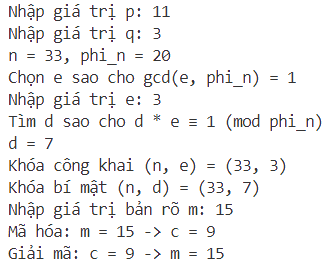
\includegraphics[scale = 0.9]{pictures/lap_trinh_vi_du_RSA.png}
\end{figure}

\end{frame}
%%%%%%%%%%%%%%%%%%%%%%%%%%%%%%%%%%%%%%%%%%%%%%%%%%%%%%%
%! %%%%%%%%%%%%%%%%%%%%%%%%%%%%%%%%%%%%%%%%%%%%%%%%%%%%%%
%! %%%%%%%%%%%%%%%%%%%%%%%%%%%%%%%%%%%%%%%%%%%%%%%%%%%%%%
%! %%%%%%%%%%%%%%%%%%%%%%%%%%%%%%%%%%%%%%%%%%%%%%%%%%%%%%
%! %%%%%%%%%%%%%%%%%%%%%%%%%%%%%%%%%%%%%%%%%%%%%%%%%%%%%%
%! %%%%%%%%%%%%%%%%%%%%%%%%%%%%%%%%%%%%%%%%%%%%%%%%%%%%%%
\section{Phương pháp lưới}
\begin{frame}{Phương pháp lưới}
\begin{itemize}
\item Phương pháp lưới là một lĩnh vực trong toán học có liên quan đến việc nghiên cứu các cấu trúc đại số và hình học của các mạng lưới được phát triển từ những năm 1940.
\item Phương pháp lưới được sử dụng trong nhiều lĩnh vực:
\begin{itemize}
\item Lĩnh vực xấp xỉ số đại số
\item Lĩnh vực mật mã học
\item Lĩnh vực khoa học máy tính
\item Lĩnh vực kỹ thuật thông tin
\end{itemize}
\end{itemize}
\end{frame}
%%%%%%%%%%%%%%%%%%%%%%%%%%%%%%%%%%%%%%%%%%%%%%%%%%%%%%%
\subsection{Định nghĩa}
\begin{frame}{Định nghĩa}
\begin{block}{Tập hợp các vector độc lập tuyến tính}
Tập hợp các vector \(\{x_1, x_2, \ldots, x_n\}\) trong \(\mathbb{R}^n\) độc lập tuyến tính nếu:

\begin{equation}
c_1 x_1 + c_2 x_2 + \ldots + c_n x_n = 0 \quad \text{với} \quad c_i \in \mathbb{R}
\end{equation}

Dấu "=" xảy ra khi và chỉ khi \(c_1 = c_2 = \ldots = c_n = 0 \).

\end{block}
\end{frame}
%%%%%%%%%%%%%%%%%%%%%%%%%%%%%%%%%%%%%%%%%%%%%%%%%%%%%%%
\begin{frame}{Định nghĩa}
\begin{block}{Cơ sở của không gian vector}
Cho \(n \geq 1 \), \(\{x_1, x_2, \ldots, x_n\}\) là một cơ sở của \(\mathbb{R}^n\).
Lưới \(n \) chiều với cơ sở \(\{x_1, x_2, \ldots, x_n\}\)
là tập hợp \(L \) tất cả các tổ hợp tuyến tính của các vector cơ sở đó với hệ số nguyên:

\begin{equation}
L = \{a_1 x_1 + a_2 x_2 + \ldots + a_n x_n \mid a_i \in \mathbb{Z} \}
\end{equation}

Các vector \(\{x_1, x_2, \ldots, x_n\}\) được gọi là cơ sở của lưới.
\end{block}
\end{frame}
%%%%%%%%%%%%%%%%%%%%%%%%%%%%%%%%%%%%%%%%%%%%%%%%%%%%%%%
\begin{frame}{Định thức}
\begin{block}{Định thức}

\end{block}
\end{frame}
%%%%%%%%%%%%%%%%%%%%%%%%%%%%%%%%%%%%%%%%%%%%%%%%%%%%%%%
\begin{frame}{Bổ đề}
\begin{block}{Bổ đề}
Cho $x_1, x_2, \ldots, x_n$ và $y_1, y_2, \ldots, y_n$ là hai cơ sở của lưới $L \subset \mathbb{R}^n$.
Lấy $X$, $Y$ lần lượt là các ma trận $n \times n$ nhận $x_i$ (tương ứng $y_i$) là các hàng thứ $i$.
Khi đó:

\begin{equation} \label{equation:bo_de}
Y = CX
\end{equation}

với $C$ là ma trận vuông $n \times n$ với các hệ số nguyên
và $\det(C) = \pm 1$.
\end{block}
\end{frame}
%%%%%%%%%%%%%%%%%%%%%%%%%%%%%%%%%%%%%%%%%%%%%%%%%%%%%%%
\begin{frame}{Bổ đề}

\textbf{Chứng minh:}

Với mọi $y_i$ thuộc lưới với cơ sở $x_1, x_2, \ldots, x_n$ và mọi $x_i$ thuộc lưới với cơ sở $y_1, y_2, \ldots, y_n$. Khi đó:
\[
x_i = \sum_{j=1}^n b_{ij} y_j, \quad y_i = \sum_{j=1}^n c_{ij} x_j.
\]

Ta có thể viết gọn lại dưới dạng ma trận:
$X = BY, \quad Y = CX.$

Vì vậy ta có $X = BCX$ và $Y = CBY$. Do $x_1, x_2, \ldots, x_n$ và $y_1, y_2, \ldots, y_n$ là cơ sở trong không gian $\mathbb{R}^n$ nên ma trận $X$, $Y$ là ma trận khả nghịch.

Suy ra $BC = CB = I$ và $\det(B) \det(C) = 1$.

Thêm nữa, $B$, $C$ là các ma trận hệ số nguyên. Do đó:
\[
\begin{cases}
\det(B) = \det(C) = 1, \\
\det(B) = \det(C) = -1.
\end{cases}
\]

\end{frame}
%%%%%%%%%%%%%%%%%%%%%%%%%%%%%%%%%%%%%%%%%%%%%%%%%%%%%%%
\begin{frame}{Nhận xét}

\begin{block}{Nhận xét}
Định thức của một lưới không phụ thuộc vào cách chọn cơ sở.
\end{block}

\textbf{Chứng minh:}

Giả sử lưới $L \subset \mathbb{R}^n$ có 2 cơ sở $x_1, x_2, \ldots, x_n$ và $y_1, y_2, \ldots, y_n$.

Theo công thức (\ref{equation:bo_de}) trong bổ đề, ta có:

\[
|\det(Y)| = |\det(CX)| = |\det(C) \cdot \det(X)| = |\pm 1 \cdot \det(X)| = |\det(X)|
\]

\end{frame}
%%%%%%%%%%%%%%%%%%%%%%%%%%%%%%%%%%%%%%%%%%%%%%%%%%%%%%%
\begin{frame}{Vector ngắn nhất}

\begin{itemize}
\item Độ dài vector $v = (v_1, v_2, \dots, v_n)$ là:

$$\|v\| = (v_1^2 + v_2^2 + \dots + v_n^2)^{\tfrac{1}{2}}$$

\item Có nhiều vấn đề liên quan đến việc tìm một vector khác không ngắn nhất trong lưới.
Bài toán tìm vector ngắn nhất (Shortest Vector Problem - SVP) rất khó để giải, khi số chiều của lưới lớn.

\end{itemize}

\end{frame}
%%%%%%%%%%%%%%%%%%%%%%%%%%%%%%%%%%%%%%%%%%%%%%%%%%%%%%%
\subsection{Trực giao hóa Gram-Schmidt}
\begin{frame}{Trực giao hóa Gram-Schmidt}
\begin{itemize}
\item Thuật toán Gram-Schmidt cổ điển chuyển một cơ sở bất kỳ trong $\mathbb{R}^n$ thành một cơ sở trực giao.
\item Đây là kỹ thuật quan trọng trong thuật toán LLL.
\end{itemize}

\begin{columns}

\begin{column}{0.5\textwidth}
\begin{figure}[h]
\centering
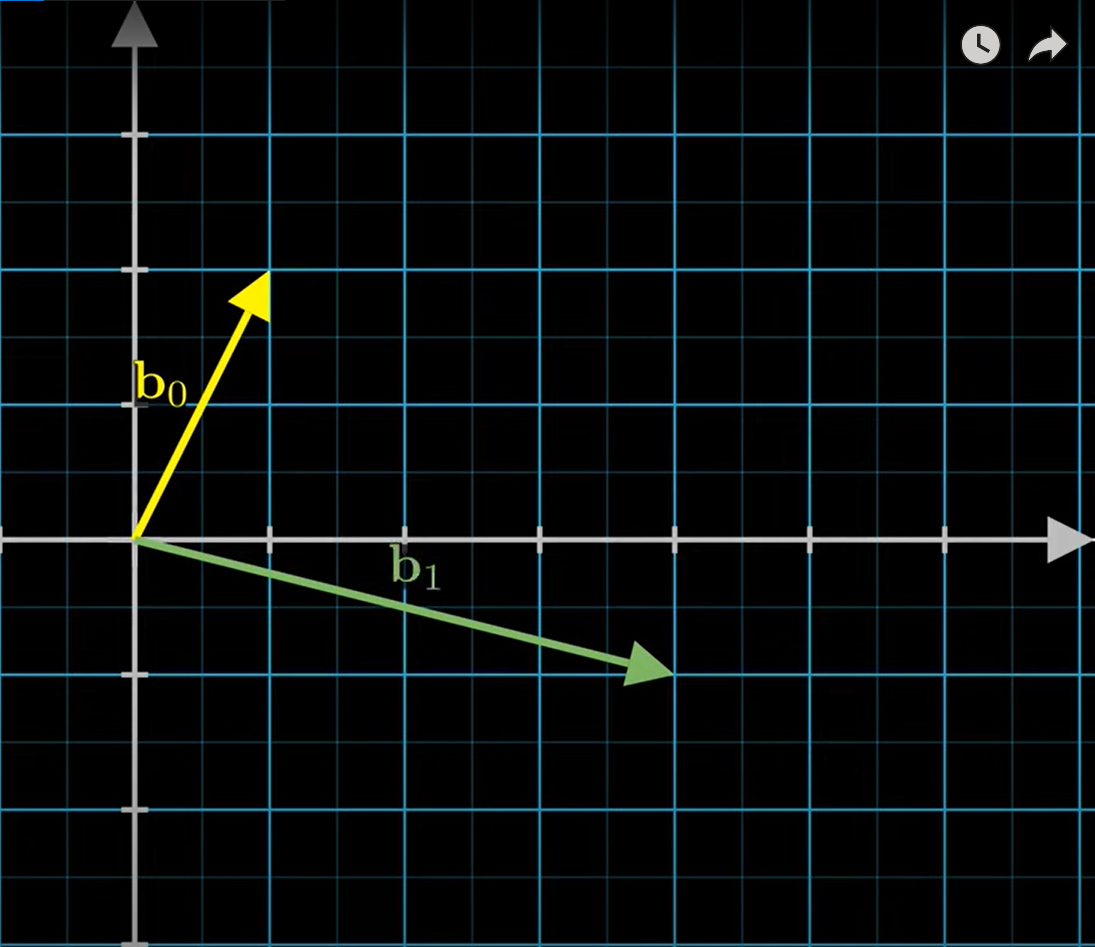
\includegraphics[width=\textwidth]{pictures/GramSchmidtYouTube0.png}
\end{figure}
\end{column}

\begin{column}{0.5\textwidth}
\begin{figure}[h]
\centering
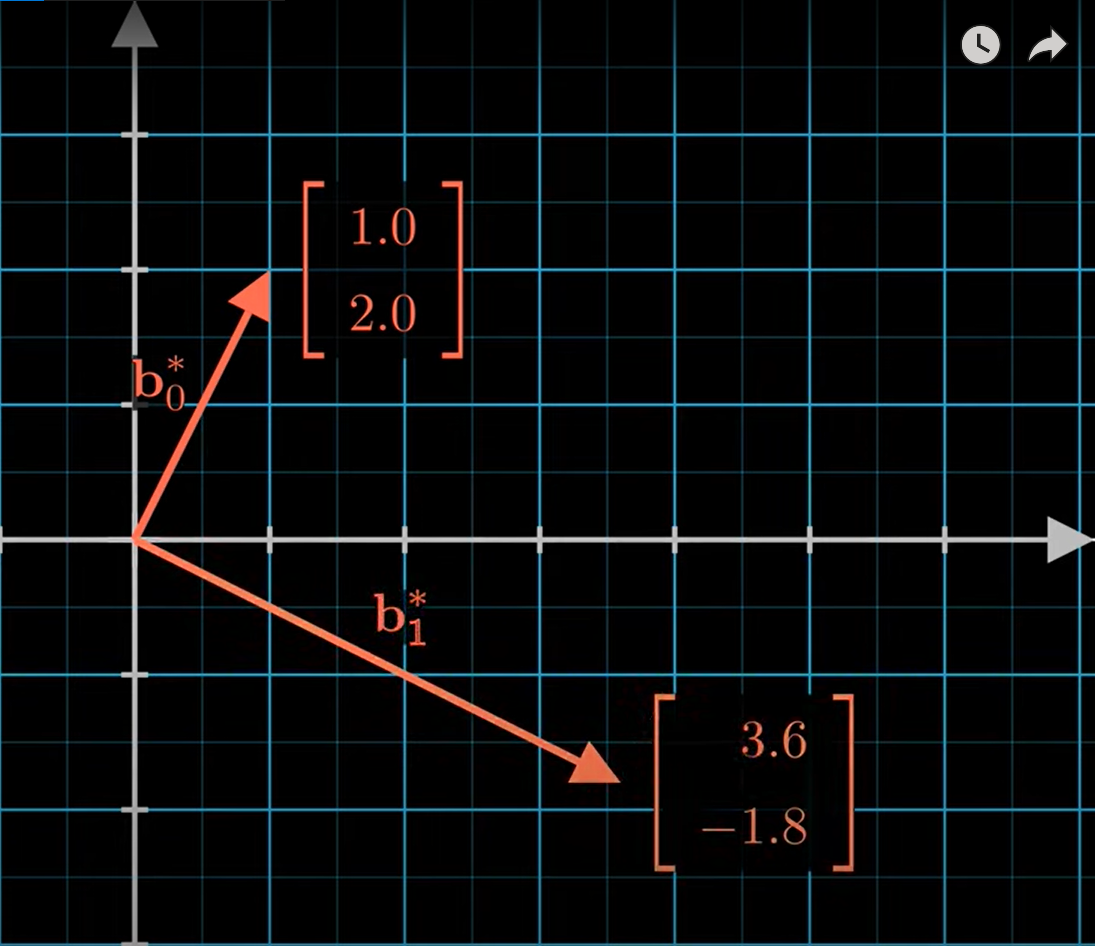
\includegraphics[width=\textwidth]{pictures/GramSchmidtYouTube1.png}
\end{figure}
\end{column}

\end{columns}

\end{frame}
%%%%%%%%%%%%%%%%%%%%%%%%%%%%%%%%%%%%%%%%%%%%%%%%%%%%%%%
\begin{frame}{Trực giao hóa Gram-Schmidt}

\begin{block}{Định nghĩa}

Cho $x_1, x_2, \ldots, x_n$ là một cơ sở trong $\mathbb{R}^n$.
Trực giao hóa Gram-Schmidt của $x_1, x_2, \ldots, x_n$
là một cơ sở $x_1^*, x_2^*, \ldots, x_n^*$ được định nghĩa như sau:

\begin{itemize}
\item $x_1 = x_1^*$,
\item $x_i^* = x_i - \sum_{j=1}^{i-1} \mu_{ij} x_j^*$, \quad $2 \leq i \leq n$, \quad $\mu_{ij} = \frac{\langle x_i, x_j^* \rangle}{\langle x_j^*, x_j^* \rangle}$.
\end{itemize}

\end{block}

\end{frame}
%%%%%%%%%%%%%%%%%%%%%%%%%%%%%%%%%%%%%%%%%%%%%%%%%%%%%%%
\begin{frame}{Ma trận}
Không hiểu?
Trang 9
Trang 10

\end{frame}
%%%%%%%%%%%%%%%%%%%%%%%%%%%%%%%%%%%%%%%%%%%%%%%%%%%%%%%
\begin{frame}{Định lý}

\begin{block}{Định lý}

Cho $x_1, x_2, \ldots, x_n$ là một cơ sở của $\mathbb{R}^n$
và $x_1^*, x_2^*, \ldots, x_n^*$ là trực giao hóa Gram-Schmidt của nó. Khi đó:

\begin{equation} \label{equation:dinh_li_Gram-Schmidt1}
\langle x_i^*, x_j^* \rangle = 0 \quad \text{với} \quad 1 \leq i < j \leq n
\end{equation}

\begin{equation} \label{equation:dinh_li_Gram-Schmidt2}
\|x_k^*\| \leq \|x_k\|
\end{equation}

\begin{equation} \label{equation:dinh_li_Gram-Schmidt3}
\det(X^*) = \det(X)
\end{equation}

\end{block}

\end{frame}
%%%%%%%%%%%%%%%%%%%%%%%%%%%%%%%%%%%%%%%%%%%%%%%%%%%%%%%
\begin{frame}{Định lý}

\textbf{Chứng minh công thức (\ref{equation:dinh_li_Gram-Schmidt1}):}
$\langle x_i^*, x_j^* \rangle = 0$ với $1 \leq i < j \leq n$

Theo định nghĩa của quá trình trực giao hóa Gram-Schmidt,
các vector $x_1^*, x_2^*, \ldots, x_n^*$ được xây dựng sao cho
mỗi vector mới là trực giao với tất cả các vector trước đó.
Cụ thể, với $x_i^*$ và $x_j^*$:

\[
x_j^* = x_j - \sum_{k=1}^{j-1} \mu_{jk} x_k^*, \quad \text{với} \quad \mu_{jk} = \frac{\langle x_j, x_k^* \rangle}{\langle x_k^*, x_k^* \rangle}
\]

Do đó, $ x_i^* x_j^* = 0$ với $1 \leq i < j \leq n$.

\end{frame}
%%%%%%%%%%%%%%%%%%%%%%%%%%%%%%%%%%%%%%%%%%%%%%%%%%%%%%%
\begin{frame}{Định lý}

\textbf{Chứng minh công thức (\ref{equation:dinh_li_Gram-Schmidt2}):}
$\|x_k^*\| \leq \|x_k\|$

Do $x_i^*$ là hình chiếu của $x_i$ lên không gian trực giao với các vector trước đó, ta có:

\[
x_i^* = x_i - \sum_{j=1}^{i-1} \mu_{ij} x_j^*
\]

Theo định lý Py-ta-go, ta có:

\[
\|x_k\|^2 = \|x_k^*\|^2 + \sum_{j=1}^{k-1} (\mu_{kj})^2 \|x_j^*\|^2.
\]

Do đó, $\|x_i^*\| \leq \|x_i\|$.

\end{frame}
%%%%%%%%%%%%%%%%%%%%%%%%%%%%%%%%%%%%%%%%%%%%%%%%%%%%%%%
\begin{frame}{Định lý}

\textbf{Chứng minh công thức (\ref{equation:dinh_li_Gram-Schmidt3}):}
$\det(X^*) = \det(X)$

% Slide ma trận
% Slide ma trận
% Slide ma trận
% Slide ma trận
% Slide ma trận
% Slide ma trận
% Slide ma trận
% Slide ma trận
% Slide ma trận
% Slide ma trận
% Slide ma trận

Theo quá trình Gram-Schmidt xxxxxxxxxxxxxxxxxxxxxxxxxxx, ta có $X = MX^*$
với $M$ là ma trận tam giác dưới với các phần tử đường chéo bằng 1 và các phần tử dưới đường chéo chính là các hệ số $\mu_{ij}$.
Ma trận $M$ có định thức bằng 1, do đó:

\[
\det(X) = \det(MX^*) = \det(M) \det(X^*) = 1 \cdot \det(X^*) = \det(X^*)
\]

\end{frame}
%%%%%%%%%%%%%%%%%%%%%%%%%%%%%%%%%%%%%%%%%%%%%%%%%%%%%%%
\begin{frame}{Bổ đề}

\begin{block}{Bổ đề}

Cho $x_1, x_2, \ldots, x_n$ là một cơ sở của $\mathbb{R}^n$
và $x_1^*, x_2^*, \ldots, x_n^*$ là trực giao hóa Gram-Schmidt của nó.
Ta có:

\[
|\det(X)| \leq \|x_1\|\|x_2\|\cdots\|x_n\|.
\]

\end{block}

\textbf{Chứng minh:}

Ta có $|\det(X^*)|$ là thể tích hình hộp $n$ chiều căng bởi các vector trực giao $x_1^*, x_2^*, \ldots, x_n^*$. Do đó:

\[
|\det(X^*)| = \|x_1^*\|\|x_2^*\|\cdots\|x_n^*\|.
\]

Theo công thức (\ref{equation:dinh_li_Gram-Schmidt2}) trong định lý, ta có:

\[
|\det(X)| = |\det(X^*)| \leq \|x_1^*\|\|x_2^*\|\cdots\|x_n^*\| \leq \|x_1\|\|x_2\|\cdots\|x_n\|.
\]

\end{frame}
%%%%%%%%%%%%%%%%%%%%%%%%%%%%%%%%%%%%%%%%%%%%%%%%%%%%%%%
%! %%%%%%%%%%%%%%%%%%%%%%%%%%%%%%%%%%%%%%%%%%%%%%%%%%%%%%
%! %%%%%%%%%%%%%%%%%%%%%%%%%%%%%%%%%%%%%%%%%%%%%%%%%%%%%%
%! %%%%%%%%%%%%%%%%%%%%%%%%%%%%%%%%%%%%%%%%%%%%%%%%%%%%%%
%! %%%%%%%%%%%%%%%%%%%%%%%%%%%%%%%%%%%%%%%%%%%%%%%%%%%%%%
%! %%%%%%%%%%%%%%%%%%%%%%%%%%%%%%%%%%%%%%%%%%%%%%%%%%%%%%
\section{Thuật toán LLL}
\begin{frame}{Thuật toán LLL}
\begin{itemize}
\item Những ứng dụng của phương pháp lưới trong hệ mật mã được phát triển từ khi có thuật toán rút gọn cơ sở lưới
\item Thuật toán rút gọn cơ sở lưới do ba nhà toán học Arjen Lenstra, Hendrik Lenstra, László Lovász tìm ra (được viết tắt là LLL) năm 1982

\end{itemize}
\end{frame}
%%%%%%%%%%%%%%%%%%%%%%%%%%%%%%%%%%%%%%%%%%%%%%%%%%%%%%%
\begin{frame}{Thuật toán LLL}
\begin{itemize}
\item Ý tưởng của việc rút gọn cơ sở là thay đổi cơ sở $B$ của lưới $L$ thành một cơ sở mới $B'$ ngắn hơn sao cho $|\det(L)|$ không đổi.
\item Từ đó sử dụng để giải bài toán vector ngắn nhất

\begin{figure}[H]
\centering
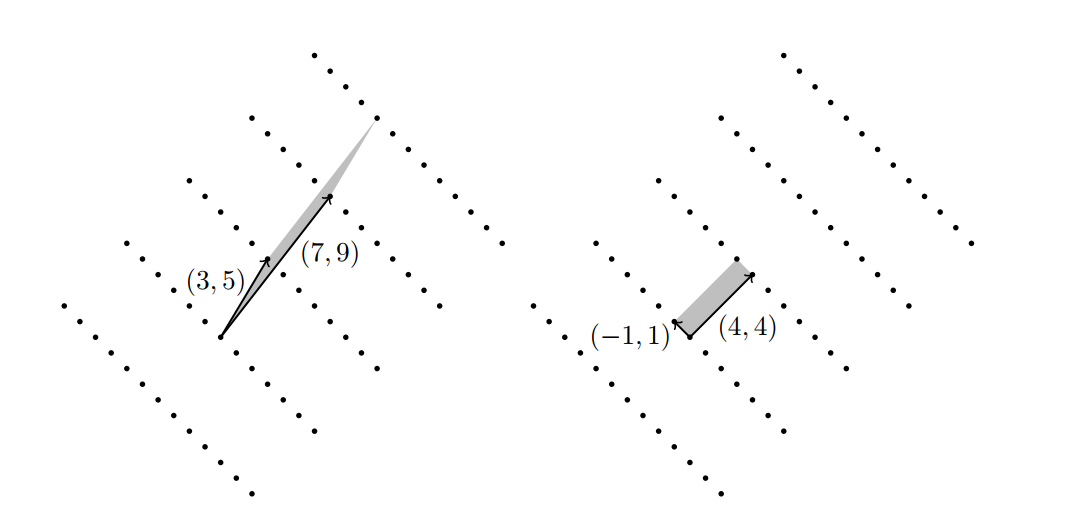
\includegraphics[scale = 0.5]{pictures/mo_ta_ket_qua_giam_luoi_LLL.png}
\caption{Lưới $L \subset R^2$. Mô tả kết quả giảm lưới trong $R^2$.}
\end{figure}

\end{itemize}
\end{frame}
%%%%%%%%%%%%%%%%%%%%%%%%%%%%%%%%%%%%%%%%%%%%%%%%%%%%%%%
\subsection{Định nghĩa}
\begin{frame}{Định nghĩa cơ sở giảm}
\begin{block}{Cơ sở giảm}

Một cơ sở $\{x_1, x_2\}$ được gọi là cơ sở giảm khi và chỉ khi:

\begin{itemize}
\item $\|x_1\| \leq \|x_2\|$,
\item $|\mu| = \left|\dfrac{x_1.x_2}{x_1.x_1}\right| \leq \dfrac{1}{2}$.
\end{itemize}

\end{block}
\end{frame}
%%%%%%%%%%%%%%%%%%%%%%%%%%%%%%%%%%%%%%%%%%%%%%%%%%%%%%%
\begin{frame}{Định lý}
\begin{block}{Định lý}
Nếu $x_1, x_2$ là cơ sở rút gọn của lưới $L$
thì $x_1$ là vector khác không ngắn nhất của lưới đó.
\end{block}

\textbf{Chứng minh:}

Đặt $ax_1 + bx_2$ là vector khác không bất kì trong lưới $L$ (với $a, b \in Z$)

Ta có: \hspace{4cm}$ \quad \|ax_1 + bx_2\|^2 = a^2\|x_1\|^2 + b^2\|x_2\|^2 + 2abx_1x_2$\\
Vì $x_1, x_2$ là cơ sở giảm nên: $$-\frac{1}{2}x_1x_1 \leq x_1x_2 \leq \frac{1}{2}x_1x_1 $$
Suy ra: \hspace{3cm} $\qquad 2abx_1x_2 \geq -|ab|\|x_1\|^2 $

\end{frame}
%%%%%%%%%%%%%%%%%%%%%%%%%%%%%%%%%%%%%%%%%%%%%%%%%%%%%%%
\begin{frame}{Định lý}

Do đó:

$$
\begin{aligned}
\|ax_1 + bx_2\|^2 &\geq a^2\|x_1\|^2 - |ab|\|x_1\|^2 + b^2\|x_2\|^2 \\
& \geq a^2\|x_1\|^2 - |ab|\|x_1\|^2 + b^2\|x_1\|^2 \quad (\text{do}\|x_2\| \geq \|x_1\|)\\
& = (a^2 - |ab| + b^2) \|x_1\|^2
\end{aligned}
$$
Ta thấy $a^2 - |ab| + b^2 \in N$ và bằng 0 khi và chỉ khi $a = b = 0$.\\
Nhưng \quad $ax_1 + bx_2 \ne 0$ \qquad $\Rightarrow$ \qquad Trường hợp $a = b = 0$ (loại).\\
\hspace*{3cm}$\Rightarrow a^2 - |ab| + b^2 \geq 1$\\
\hspace*{3cm}$ \Rightarrow \|ax_1 + bx_2\| \geq \|x_1\|^2$.\\
Do đó $x_1$ là vector khác không ngắn nhất của lưới.
\end{frame}
%%%%%%%%%%%%%%%%%%%%%%%%%%%%%%%%%%%%%%%%%%%%%%%%%%%%%%%
\subsection{Giảm lưới 2 chiều}
\begin{frame}{Giảm lưới 2 chiều}
\begin{itemize}
\item Việc giảm cơ sở lưới 2 chiều tương đối dễ hiểu.
\item Đặt $\{x_1, x_2\}$ làm cơ sở của lưới 2 chiều.
\item Mục tiêu của chúng ta sẽ thay thế cơ sở này bằng cơ sở giảm.
\begin{enumerate}
\item Nếu $\|x_1\| > \|x_2\|$ ta sẽ hoán vị $x_1$ với $x_2$.
\item Thay vector $x_2$ bằng vector $x_2^*$ vuông góc với $x_1$ qua phép trực giao hóa Gram-Schmidt :
$$x_2^* = x_2 - \frac{x_1.x_2}{x_1.x_1}.x_1 $$ Đặt $t$ là số nguyên gần nhất với $\dfrac{x_1.x_2}{x_1.x_1}$
\item Ta thay thế cơ sở $\{x_1, x_2 \}$ bằng cơ sở $$\{x_1, x_2 - tx_1\}$$
\item Lặp lại quy trình này đến khi không thể giảm cơ sở nữa.
\end{enumerate}
\end{itemize}
\end{frame}
%%%%%%%%%%%%%%%%%%%%%%%%%%%%%%%%%%%%%%%%%%%%%%%%%%%%%%%
\begin{frame}{Ví dụ giảm lưới 2 chiều}

\begin{block}{Ví dụ giảm lưới 2 chiều}
Cho $\{x_1, x_2\}$ là cơ sở của lưới $L$ với $x_1 = (31, 59), x_2 = (37, 70)$. Thực hiện giảm cơ sở lưới trên.
\end{block}

\begin{itemize}
\item Với: $x_1 = (31, 59), x_2 = (37, 70)$
\item Ta có: $\|x_1\|= \sqrt{4442}$ và $\|x_2\| = \sqrt{6269}$ $\Rightarrow$ $\|x_1\| \leq \|x_2\|$
\item Và: $\dfrac{x_1.x_2}{x_1.x_1} = \dfrac{5277}{4442} \approx 1, 18$
\item Chọn $t = 1 $ suy ra cơ sở mới:

$$\begin{cases}
x_1^{*} = x_1 = (31, 59)\\
x_2^{*} = x_2 - t x_1 = (6, 11)
\end{cases}$$
\end{itemize}

\end{frame}
%%%%%%%%%%%%%%%%%%%%%%%%%%%%%%%%%%%%%%%%%%%%%%%%%%%%%%%
\begin{frame}{Ví dụ giảm lưới 2 chiều}
\begin{itemize}
\item Với: $x_1 = (31, 59), x_2 = (6, 11)$
\item Ta có: $\|x_1\|= \sqrt{4442}$ và $\|x_2\| = \sqrt{157}$ $\Rightarrow$ $\|x_1\| \geq \|x_2\|$

Hoán vị 2 vector ta có:

$$\begin{cases}
x_1 = (6, 11)\\
x_2 = (31, 59)
\end{cases}$$

\item Và: $\dfrac{x_1.x_2}{x_1.x_1} = \dfrac{835}{157} \approx 5, 3$

\item Chọn $t = 5$ ta có cơ sở mới:

$$\begin{cases}
x_1^{*} = x_1 = (6, 11) \\
x_2^{*} = x_2 - t x_1 = (1, 4)
\end{cases}$$

\end{itemize}

\end{frame}
%%%%%%%%%%%%%%%%%%%%%%%%%%%%%%%%%%%%%%%%%%%%%%%%%%%%%%%
\begin{frame}{Ví dụ giảm lưới 2 chiều}
\begin{itemize}

\item Với: $x_1 = (6, 11), x_2 = (1, 4)$
\item Ta có: $\|x_1\|= \sqrt{157}$ và $\|x_2\| = \sqrt{17}$ $\Rightarrow$ $\|x_1\| \geq \|x_2\|$

Hoán vị 2 vector ta có:

$$\begin{cases}
x_1 = (1, 4)\\
x_2 =(6, 11)
\end{cases}$$

\item Và: $\dfrac{x_1.x_2}{x_1.x_1} = \dfrac{50}{17} \approx 2, 9$

\item Chọn $t = 3$ ta có cơ sở mới:

$$\begin{cases}
x_1^{*} = x_1 = (1, 4)\\
x_2^{*} = x_2 - t x_1 = (3, -1)
\end{cases}$$

\end{itemize}
\end{frame}
%%%%%%%%%%%%%%%%%%%%%%%%%%%%%%%%%%%%%%%%%%%%%%%%%%%%%%%
\begin{frame}{Ví dụ giảm lưới 2 chiều}
\begin{itemize}

\item Với: $x_1 = (1, 4), x_2 = (3, -1)$
\item Ta có: $\|x_1\|= \sqrt{17}$ và $\|x_2\| = \sqrt{10}$ $\Rightarrow$ $\|x_1\| \geq \|x_2\|$

Hoán vị 2 vector ta có:

$$\begin{cases}
x_1 = (3, -1)\\
x_2 = (1, 4)
\end{cases}$$

\item Và: $\dfrac{x_1.x_2}{x_1.x_1} = -\dfrac{1}{10}$

\end{itemize}

$\Rightarrow$ Suy ra cơ sở giảm của lưới $L$ là $\{(3, -1), (1, 4)\}$

\end{frame}
%%%%%%%%%%%%%%%%%%%%%%%%%%%%%%%%%%%%%%%%%%%%%%%%%%%%%%%
\begin{frame}{Thuật toán giảm lưới 2 chiều}

\begin{enumerate}
\item Nhập vào cơ sở lưới 2 chiều ${b_1, b_2} \in R^2$.
\item Nếu $\|b_1\| > \|b_2\|$, ta hoán đổi vị trí $b_1$ và $b_2$.
\item Đặt $t$ bằng phần nguyên $\left|\dfrac{b_1.b_2}{b_1.b_1}\right|$

% # phần nguyên thì sao ví dụ 2, 9 =>3??
% # phần nguyên thì sao ví dụ 2, 9 =>3??
% # phần nguyên thì sao ví dụ 2, 9 =>3??
% # phần nguyên thì sao ví dụ 2, 9 =>3??
% # phần nguyên thì sao ví dụ 2, 9 =>3??
% # phần nguyên thì sao ví dụ 2, 9 =>3??
% # phần nguyên thì sao ví dụ 2, 9 =>3??
% # phần nguyên thì sao ví dụ 2, 9 =>3??

Nếu $t = 0$, dừng lại và kết luận là cơ sở giảm.

Ngược lại, ta tính lại $b_2 = b_2 - t.b_1$ và quay lại bước 2
\end{enumerate}

\end{frame}
%%%%%%%%%%%%%%%%%%%%%%%%%%%%%%%%%%%%%%%%%%%%%%%%%%%%%%%
\begin{frame}{Thuật toán giảm lưới 2 chiều}

\begin{figure}[h]
\centering
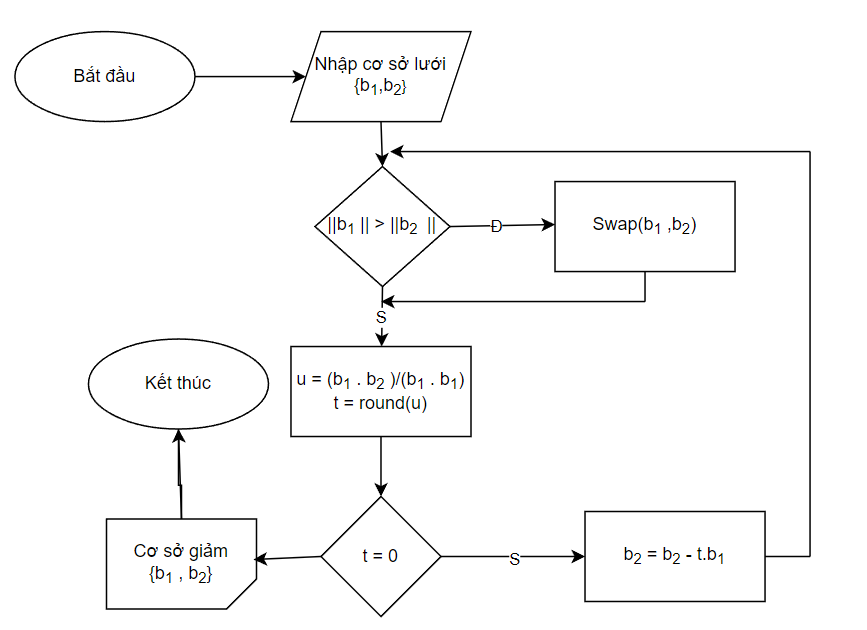
\includegraphics[scale = 0.6]{pictures/thuat_toan_giam_luoi_2_chieu.png}
\end{figure}

\end{frame}
%%%%%%%%%%%%%%%%%%%%%%%%%%%%%%%%%%%%%%%%%%%%%%%%%%%%%%%
\subsection{Thuật toán giảm lưới nhiều chiều}
\begin{frame}{Thuật toán giảm lưới nhiều chiều}
\begin{itemize}
\item Việc giảm cơ sở lưới nhiều chiều khó khăn hơn nhiều
\item Thuật toán LLL sử dụng cách tiếp cận tìm kiếm các vector gần như ngắn nhất (trong thời gian đa thức)
\end{itemize}
\end{frame}
%%%%%%%%%%%%%%%%%%%%%%%%%%%%%%%%%%%%%%%%%%%%%%%%%%%%%%%
\begin{frame}{Định nghĩa}

\begin{block}{Định nghĩa}

Tham số rút gọn $\alpha$ là một số thực sao cho $\dfrac{1}{4} < \alpha < 1$.
Giá trị chính tắc của $\alpha$ là $\alpha = \dfrac{3}{4}$

\end{block}

\begin{block}{Định nghĩa}

Cơ sở $x_1, x_2, \dots, x_n$ được gọi là một cơ sở $\alpha$-rút gọn nếu nó thỏa mãn:

\begin{itemize}
\item $|\mu_{ij}| \leq \dfrac{1}{2} $ với $1 \leq j < i \leq n$,
\item $\|x_i^*\|^2 \geq (\alpha - \mu_{i, i-1}^2)\|x_{i-1}^*\|^2$ với $2\leq i \leq n$.
\end{itemize}

\end{block}

Ta định nghĩa tham số bổ trợ $\beta$ như sau: \quad $\beta = \dfrac{4}{4\alpha - 1}$.

Do \quad $\frac{1}{4} < \alpha < 1$ \quad $\Rightarrow \quad \beta > \dfrac{4}{3}$. \quad Nếu $\alpha = \dfrac{3}{4}$ thì $\beta = 2$.

\end{frame}
%%%%%%%%%%%%%%%%%%%%%%%%%%%%%%%%%%%%%%%%%%%%%%%%%%%%%%%
\begin{frame}{Mệnh đề}

\begin{block}{Mệnh đề}

Nếu $x_1, x_2, \dots, x_n$ là một cơ sở $\alpha$-rút gọn của lưới $L$ trong $R^n$
và $x_1^*, x_2^*, \dots, x_n^*$ là cơ sở trực giao hóa Gram-Schmidt của nó thì:

\begin{equation} \label{equation:menh_de_thua_toan_giam_luoi_nhieu_chieu1}
\|x_j\|^2 \leq \beta^{i-1}\|x_i^*\|^2 \quad \text{với} \quad 1 \leq j \leq i \leq n
\end{equation}

\begin{equation} \label{equation:menh_de_thua_toan_giam_luoi_nhieu_chieu2}
\|x_1\|.\|x_2\|\dots\|x_n\| \leq \beta^{\tfrac{n(n-1)}{4}}det(L)
\end{equation}

\begin{equation} \label{equation:menh_de_thua_toan_giam_luoi_nhieu_chieu3}
\|x_1\| \leq \beta^{\tfrac{(n-1)}{4}}det(L)^{\frac{1}{n}}
\end{equation}

\end{block}

\end{frame}
%%%%%%%%%%%%%%%%%%%%%%%%%%%%%%%%%%%%%%%%%%%%%%%%%%%%%%%
\begin{frame}{Mệnh đề}

\textbf{Chứng minh công thức (\ref{equation:menh_de_thua_toan_giam_luoi_nhieu_chieu1}):}
$\|x_j\|^2 \leq \beta^{i-1}\|x_i^*\|^2$ với $1 \leq j \leq i \leq n $

% \textit{Chứng minh.}\\
% i) Theo Định nghĩa 2.7 ta có :
% $$\|x_i^*\| \geq (\alpha - \mu_{i, i-1}^2)\|x_{i-1}^*\|^2 \geq (\alpha - \frac{1}{4}).\|x_{i-1}^*\|^2 = \frac{1}{\beta}\|x_{i-1}^*\|^2 \text{.}$$
% Khi đó \quad $\|x_{i-1}^*\|^2 \leq \beta.\|x_{i}^*\|^2$, và $$\|x_{j}^*\|^2 \leq \beta^{i-j}\|x_{i}^*\|^2 \qquad (1 \leq j \leq i \leq n)\text{.} \qquad (1)$$
% Mặt khác, ta có : $$x_i = x_i^* + \displaystyle\sum_{j=1}^{i-1} \mu_{ij}x_j^*\text{,}$$ và vì $x_1^*, x_2^*, \dots, x_n^*$ là trực giao nên:
% $$
% \begin{aligned}
% \|x_i\|^2 & = \|x_i^*\|^2 + \displaystyle\sum_{j=1}^{i-1} (\mu_{ij})^2\|x_j^*\|^2 \leq \|x_i^*\|^2 + \displaystyle\sum_{j=1}^{i-1} \frac{1}{4}\beta^{i-j}\|x_i^*\|^2\\
% & \leq (1 + \frac{1}{4}\displaystyle\sum_{j=1}^{i-1} \beta^{i-j})\|x_i^*\|^2 = (1 + \frac{1}{4}\frac{\beta^i - \beta}{\beta - 1})\|x_i^*\|^2 \text{.}
% \end{aligned}
% $$
% Bằng quy nạp, ta có thể dễ chứng minh $$1 + \frac{1}{4}\frac{\beta^i - \beta}{\beta - 1} \leq \beta^{i-1}.$$
% Vì vậy,
% $$ \|x_i\|^2 \leq \beta^{i-1}\|x_i^*\|^2 \text{.} \qquad\qquad (2)$$
% Từ (1), (2) ta có:\\
% \hspace*{4cm} $\|x_j\|^2 \leq \beta^{j-1}\|x_j^*\|^2 \leq \beta^{i-1}\|x_i\|^2 \text{.}$\\

\end{frame}
%%%%%%%%%%%%%%%%%%%%%%%%%%%%%%%%%%%%%%%%%%%%%%%%%%%%%%%
\begin{frame}{Mệnh đề}

\textbf{Chứng minh công thức (\ref{equation:menh_de_thua_toan_giam_luoi_nhieu_chieu2}):}
$\|x_1\|.\|x_2\|\dots\|x_n\| \leq \beta^{\tfrac{n(n-1)}{4}}det(L) $

% ii) Theo Bổ đề 2.3. ta có :
% $$det(L) = \|x_1^*\|.\|x_2^*\|\dots\|x_n^*\| \leq \|x_1\|.\|x_2\|\dots\|x_n\|\text{.}$$
% Từ (2) ta có: \\
% \hspace*{2cm}$\qquad \|x_1\|.\|x_2\|\dots\|x_n\| \leq \beta^{\tfrac{n(n-1)}{4}}\|x_1^*\|.\|x_2^*\|\dots\|x_n^*\| = \beta^{\tfrac{n(n-1)}{4}}.det(L)$\\

\end{frame}
%%%%%%%%%%%%%%%%%%%%%%%%%%%%%%%%%%%%%%%%%%%%%%%%%%%%%%%
\begin{frame}{Mệnh đề}

\textbf{Chứng minh công thức (\ref{equation:menh_de_thua_toan_giam_luoi_nhieu_chieu3}):}
$\|x_1\| \leq \beta^{\tfrac{(n-1)}{4}}det(L)^{\frac{1}{n}} $

% iii) Xét $j = 1$ trong i), ta có $$\|x_1\|^2 \leq \beta^{i-1}\|x_i^*\|^2 $$ với $1\leq i \leq n$.

% \noindent Khi đó: $$\qquad \|x_1\|^{2n} \leq \beta^{0 + 1 +2 + \dots +(n-1)}\|x_1^*\|^2.\|x_2^*\|^2\dots\|x_n^*\|^2 \leq \beta^{\tfrac{n(n-1)}{2}}.det(L)^2\text{.}$$

% \noindent Suy ra:
% $$ \qquad \|x_1\| \leq \beta^{\tfrac{n-1}{4}}.det(L)^{\tfrac{1}{n}}\text{.}$$
% \hspace{2cm}

\end{frame}
%%%%%%%%%%%%%%%%%%%%%%%%%%%%%%%%%%%%%%%%%%%%%%%%%%%%%%%
\begin{frame}{Bổ đề}

\begin{block}{Bổ đề}

\end{block}

% \defi{\textbf{Bổ đề 2.9.} \textit{Cho $x_1, x_2, \dots, x_n$ là một cơ sở \index{cơ sở} của lưới $L$ và $x_1^*, x_2^*, \dots, x_n^*$ tương ứng là phép trực giao hóa Gram-Schmidt của nó. Với $y \in L$ khác không, $$\|y\| \geq min\{\|x_1^*\|, \|x_2^*\|, \dots, \|x_n^*\|\}\text{.}$$}}

% \textit{Chứng minh.}\\
% Cho $y$ là vector khác không bất kỳ thuộc lưới $L$ ta có : $$y = a_1x_1 + a_2x_2 + \dots + a_nx_n \text{.}$$
% Lấy $k$ là chỉ số lớn nhất sao cho $a_k \ne 0$. Khi đó:
% $$
% \begin{aligned}
% y & = \displaystyle\sum_{i=1}^{k} a_i.\displaystyle\sum_{j=1}^{i} \mu_{ij}x_j^* = \displaystyle\sum_{i=1}^{k}\displaystyle\sum_{j=1}^{i}a_i.\mu_{ij}.x_j^*\\
% & = \displaystyle\sum_{i=1}^{k}\left(\displaystyle\sum_{j=1}^{i} a_i.\mu_{ij}\right)x_j^* = a_k.x_k^* + \displaystyle\sum_{j=1}^{k-1} v_jx_j^*\text{.}
% \end{aligned}
% $$
% Khi đó: $$\|y\| \geq a_k^2.\|x_k^*\|^2 + \displaystyle\sum_{j=1}^{k-1} v_j^2\|x_j^*\|^2 .$$
% Mặt khác, do $a_k$ nguyên và khác 0 nên $a_k^2 \geq 1$:
% $$\Rightarrow \quad \|y\| \geq \|x_k^*\|^2 + \displaystyle\sum_{j=1}^{k-1} v_j^2\|x_j^*\|^2 \text{.}$$
% Vì vậy: $$\|y\|\geq \|x_k^*\| \geq min\{\|x_1^*\|, \|x_2^*\|, \dots, \|x_n^*\|\}.$$
% Ta có điều phải chứng minh.
% \vspace{0.2cm}

\end{frame}
%%%%%%%%%%%%%%%%%%%%%%%%%%%%%%%%%%%%%%%%%%%%%%%%%%%%%%%
\begin{frame}{Định lý}

\begin{block}{Định lý}

\end{block}

% \defi{\textbf{Định lý 2.10.} \textit{Nếu $x_1, x_2, \dots, x_n$ là một cơ sở $\alpha$-rút gọn của lưới $L$ trong $R^n$ và $y\in L$ là vector trong lưới khác không bất kỳ thì: $$\|x_1\| \leq \beta^{\frac{n-1}{2}}\|y\|\text{.}$$
% Đặc biệt, vector đầu tiên trong cơ sở rút gọn không dài hơn $\beta^{\tfrac{n-1}{2}}$ lần vector ngắn nhất \index{vector ngắn nhất} khác không của lưới \index{lưới} $L$.}}

% \textit{Chứng minh.}\\
% Ta có $\|x_i^*\| \geq \frac{1}{\beta}\|x_{i-1}^*\|$ với $1\leq i \leq n$. Vì $x_1^* = x_1$ nên $$\|x_1\|^2 = \|x_1^*\| \leq \beta^{n-1}\|x_n^*\|.$$
% Do đó, với $1\leq i \leq n$ ta có : $$\|x_i^*\|^2 \geq \beta^{-(i-1)}\|x_1\|^2.$$
% Theo Bổ đề 2.9, với vector khác 0 bất kì $y \in L$ ta có:
% $$\|y\| \geq \min\{\|x_1^*\|, \|x_2^*\|, \dots, \|x_n^*\|\} \geq \beta^{\tfrac{-(n-1)}{2}}\|x_1^*\| . $$
% Vì vậy, ta có điều phải chứng minh
% \vspace{0.5cm}

\end{frame}
%%%%%%%%%%%%%%%%%%%%%%%%%%%%%%%%%%%%%%%%%%%%%%%%%%%%%%%

%%%%%%%%%%%%%%%%%%%%%%%%%%%%%%%%%%%%%%%%%%%%%%%%%%%%%%%
%%%%%%%%%%%%%%%%%%%%%%%%%%%%%%%%%%%%%%%%%%%%%%%%%%%%%%%
%%%%%%%%%%%%%%%%%%%%%%%%%%%%%%%%%%%%%%%%%%%%%%%%%%%%%%%
%%%%%%%%%%%%%%%%%%%%%%%%%%%%%%%%%%%%%%%%%%%%%%%%%%%%%%%
%%%%%%%%%%%%%%%%%%%%%%%%%%%%%%%%%%%%%%%%%%%%%%%%%%%%%%%

%%%%%%%%%%%%%%%%%%%%%%%%%%%%%%%%%%%%%%%%%%%%%%%%%%%%%%%

%%%%%%%%%%%%%%%%%%%%%%%%%%%%%%%%%%%%%%%%%%%%%%%%%%%%%%%

% \defi{\textbf{Thuật toán LLL.}}
% \begin{itemize}
% \item Bước 1 : Nhập vào lưới $L$ với cơ sở lưới $b_1, b_2, \dots, b_n$ và tham số bổ trợ $c$ với $c \geq \dfrac{4}{3}$.
% \item Bước 2 : Tính cơ sở trực giao hóa Gram-Schmidt $b_1^*, b_2^*, \dots, b_n^*$ và các hệ số trực giao $u_{ij}$.
% \item Bước 3 : Thực hiện vòng lặp, nếu $\|b_i^*\|^2 \leq c.\|b_{i+1}^*\|^2$ tăng $i$ lên, ngược lại thực hiện hoán vị các vector $b_i$ và $b_{i+1}$, sau đó cập nhật lại cơ sở trực giao Gram-Schmidt và các hệ số của nó. \\
% Kiểm tra xem hệ số $\|u_{ij}\| > \dfrac{1}{2}$ thực hiện thủ tục rút gọn.\\
% Kết quả cuối cùng thu được cơ sở lưới giảm $L$.
% \item Thủ tục rút gọn: Ta sẽ rút gọn vector $b_i$ bằng cách trừ đi một bội nguyên $\|u_{ij}\|$ của $b_j$. Vì $\|u_{ij}\|$ là số nguyên gần nhất với hệ số Gram-Schmidt $u_{ij}$ nên đây là phép rút gọn tốt nhất ta có thể thực hiện, với điều kiện ràng buộc là $b_i$ vẫn nằm trong lưới ban đầu. Và cập nhật các hệ số cơ sở Gram-Schmidt.

% \end{itemize}
% \vspace{1cm}
% \noindent Sau đây là lưu đồ mô tả cách hoạt động của thuật toán LLL.
% \begin{figure}[h!]
% \centering
% 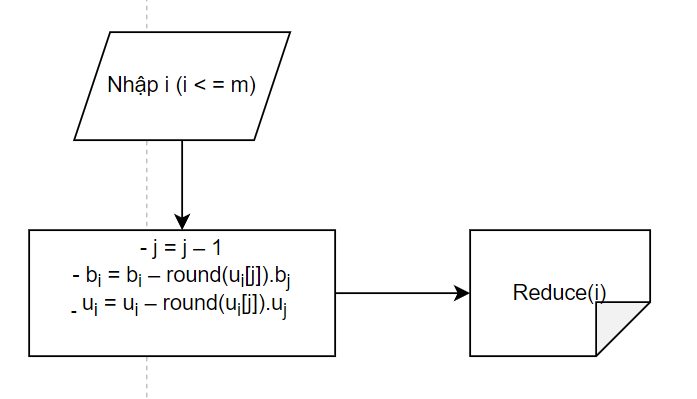
\includegraphics[scale = 1.1]{a.12.png}
% \caption{Hàm reduce.}
% \label{fig:boat1}
% \end{figure}
% \newpage
% \begin{figure}[h!]
% \centering
% 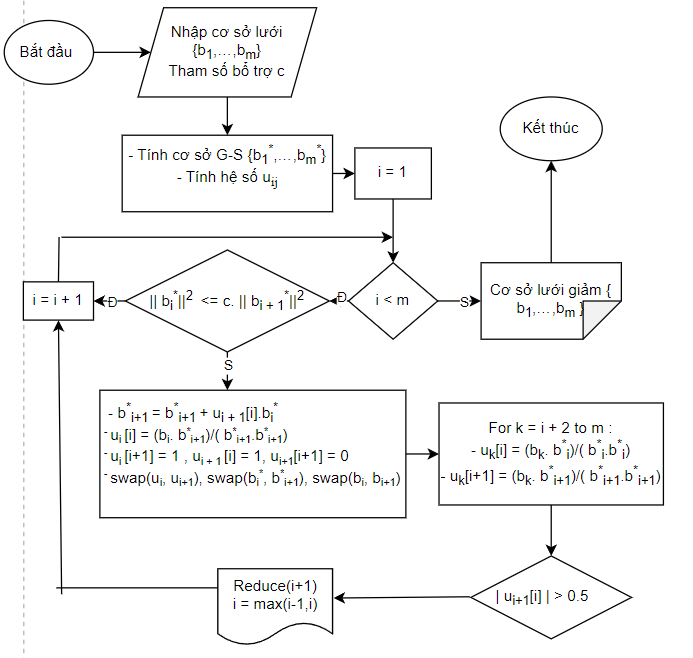
\includegraphics[width = 1\textwidth]{a.11.3.png}
% \caption{Thuật toán LLL.}
% \label{fig:boat1}
% \end{figure}
% % \begin{figure}[h!]
% % \centering
% % 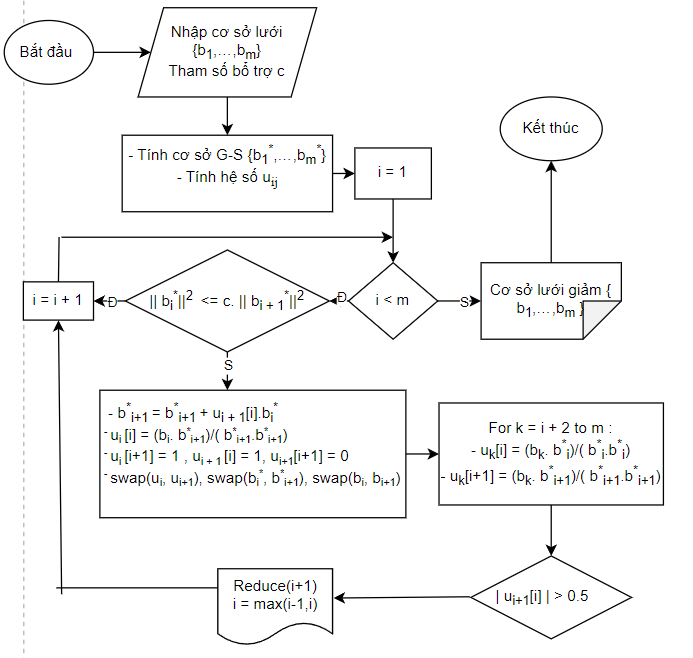
\includegraphics[scale = 1.3]{a.11.3.png}
% % \caption{Thuật toán LLL}
% % \label{fig:boat1}
% % \end{figure}
% % Trong đó, hàm Reduce có thuật toán sau :\\

% \section{Thực hiện chương trình}
% Để triển khai và kiểm tra các thuật toán, bài báo cáo này sẽ sử dụng phần mềm SageMath \index{SageMath}. SageMath là một chương trình tính toán mã nguồn mở, cấp phép bởi GPL. Nó là sự kết hợp sức mạnh của nhiều gói source vào Python (NumPy, SciPy, matplotlib, Sympy, Maxima, GAP, FLINT, R and many more). Nhiệm vụ của Sage là tạo ra một chương trình miễn phí có thể thay thế Magma, Maple, Mathematica và Matlab. Trang web \href{https://www.sagemath.org/}{https://www.sagemath.org/}.
% \vspace{1cm}\\
% Chương trình thuật toán LLL:\\

% \begin{lstlisting}
% #Ham giam luoi
% def reduce(i, B, U):

% print("gia tri ma tran B: \n")
% j = i - 1
% while j >= 0:
% B.set_column(i, B.column(i) - round(U[j, i]) * B.column(j))
% U.set_column(i, U.column(i) - round(U[j, i]) * U.column(j))
% j = j - 1
% print(B)

% #ham chinh gia tri ma tran bang thuat toan LLL
% def LLL(B, c=2):
% #Lay so hang va cot ma tran
% n = B.nrows()
% m = B.ncols()
% #khoi tao ma tran
% U = matrix(RR, m, m)
% O = matrix(RR, n, m)

% # Truc giao hoa G-S
% for i in range(0, m):
% U[i, i] = 1
% O.set_column(i, B.column(i))
% for j in range(0, i):
% U[j, i] = (B.column(i) * O.column(j)) / (O.column(j) * O.column(j))
% O.set_column(i, O.column(i) - U[j, i] * O.column(j))
% reduce(i, B, U) # Goi ham recduce de bien doi ma tran
% i += 1

% # Dieu kien giam
% i = 0
% while i < m - 1:
% if O.column(i) * O.column(i) <= c * O.column(i + 1) * O.column(i + 1):
% i += 1
% else:
% O.set_column(i + 1, O.column(i + 1) + U[i, i + 1] * O.column(i))
% U[i, i] = (B.column(i) * O.column(i + 1)) / (O.column(i + 1) * O.column(i + 1))
% U[i + 1, i] = 1
% U[i, i + 1] = 1
% U[i + 1, i + 1] = 0
% O.set_column(i, O.column(i) - U[i, i] * O.column(i + 1))
% U.swap_columns(i, i + 1)
% O.swap_columns(i, i + 1)
% B.swap_columns(i, i + 1)
% for k in range(i + 2, m):
% U[i, k] = (B.column(k) * O.column(i)) / (O.column(i) * O.column(i))
% U[i + 1, k] = (B.column(k) * O.column(i + 1)) / (O.column(i + 1) * O.column(i + 1))
% if abs(U[i, i + 1]) > 0.5:
% reduce(i + 1, B, U)
% i = max(i - 1, 0)
% return B

% # Nhap du lieu tu ban phim

% n = int(input("Nhap so chieu cua luoi n: "))
% A = Matrix(ZZ, n, n)
% for j in range(n):
% row = input(f"Nhap hang {j+1} cua ma tran : ")
% A[j] = list(map(int, row.split()))
% print(A)
% print("Ket qua giam luoi:\n")
% res = LLL(A)

% \end{lstlisting}

% \newpage

% \noindent \textbf{Một số kết quả thu được.}

% \begin{enumerate}
% \item \textbf{Lưới 2 chiều:} Cho cơ sở $x_1 = (2, 5), x_2 = (5, 8)$ :
% \begin{figure}[h!]
% \centering
% \includegraphics[width = 0.6\textwidth]{a.6.png}
% \caption{Chương trình thuật toán LLL với lưới 2 chiều.}
% \label{fig:boat1}
% \end{figure}
% % Lưới sau khi rút gọn có cơ sở mởi $x_1 = (1, -2), x_2 = (4, 1)$.
% % \begin{figure}[h!]
% % \centering
% % \includegraphics[scale = 1.1]{a.6.png}

% % \label{fig:boat1}
% % \end{figure}
% \item \textbf{Lưới 3 chiều:} Cho cơ sở $x_1 = (1, 1, 1), x_2 = (-1, 0, 2), x_3 = (3, 5, 6)$:
% \begin{figure}[h!]
% \centering
% \includegraphics[width = 0.5\textwidth]{a.7.png}
% \caption{Chương trình thuật toán LLL với lưới 3 chiều.}
% \label{fig:boat1}
% \end{figure}
% \end{enumerate}

%! %%%%%%%%%%%%%%%%%%%%%%%%%%%%%%%%%%%%%%%%%%%%%%%%%%%%%%
%! %%%%%%%%%%%%%%%%%%%%%%%%%%%%%%%%%%%%%%%%%%%%%%%%%%%%%%
%! %%%%%%%%%%%%%%%%%%%%%%%%%%%%%%%%%%%%%%%%%%%%%%%%%%%%%%
%! %%%%%%%%%%%%%%%%%%%%%%%%%%%%%%%%%%%%%%%%%%%%%%%%%%%%%%
%! %%%%%%%%%%%%%%%%%%%%%%%%%%%%%%%%%%%%%%%%%%%%%%%%%%%%%%
% \section{Ứng dụng phương pháp lưới trong hệ mật mã RSA}
% \begin{frame}{Ứng dụng phương pháp lưới trong hệ mật mã RSA}
% \begin{block}{Bài toán}
% Bài toán RSA với số mũ $e$ nhỏ, $m$ có giá trị lớn. Cho $m^e$, ta có $B$ với $|m-B| \leq n^{\tfrac{1}{e}}$. Tìm $m \in Z_n$
% \end{block}

% \end{frame}
% %%%%%%%%%%%%%%%%%%%%%%%%%%%%%%%%%%%%%%%%%%%%%%%%%%%%%%%
% \subsection{Ví dụ ứng dụng}
% \begin{frame}{Ví dụ ứng dụng}

% Trong bài toán này, thông báo có dạng $m = B + x$, trong đó $B$ cố định và $|x| \leq Y$ với Y nguyên

% Giả sử Bob có khóa công khai $(n, e) = (n, 3)$

% Khi đó bài toán là $c \equiv (B+x)^3 \quad (mod \ n)$
% \end{frame}
% %%%%%%%%%%%%%%%%%%%%%%%%%%%%%%%%%%%%%%%%%%%%%%%%%%%%%%%
% \begin{frame}{Ví dụ ứng dụng}

% Ta giả sử rằng Eve biết $B, Y, n$ . Vì vậy cô ấy chỉ cần tìm $x$. Ta có thể tạo thành đa thức:
% $$
% \begin{aligned}
% f(T) & = (B+T)^3 - c = T^3 + 3BT^2 + 3B^2T + B^3 -c\\
% & \equiv T^3 + a_2T^2 + a_1T + a_0 (mod \ n).
% \end{aligned}
% $$

% Eve đang tìm $|x| \leq Y$ sao cho $f(x) \equiv 0 \quad (mod \ n)$. Nói cách khác, cô ấy đang tìm nghiệm nhỏ của đồng dư đa thức $f(T) \equiv 0 \quad (mod \ n)$
% \end{frame}
% %%%%%%%%%%%%%%%%%%%%%%%%%%%%%%%%%%%%%%%%%%%%%%%%%%%%%%%
% \begin{frame}{Ví dụ ứng dụng}

% Eve áp dụng thuật toán LLL cho lưới được tạo bởi các vector:
% $$v_1 =(n, 0, 0, 0), v_2 = (0, Yn, 0, 0) $$
% $$ v_3 = (0, 0, Y^2n, 0), v_4 = (a_0, a_1Y, a_2Y^2, Y^3)$$
% Điều này tạo nên cơ sở mới $b_1, b_2, b_3, b_4$ . Nhưng ở đây, ta chỉ quan tâm đến $b_1$. Theo Mệnh đề 2.8 ta có
% $$
% \begin{aligned}
% \|b_1\| & \leq 2^{\tfrac{3}{4}}.det(v_1, \dots, v_4)^{\tfrac{1}{4}} \qquad \quad \text{với} \quad \alpha = \frac{3}{4} \quad \text{hay} \quad \beta = 2 \\
% & = 2^{\tfrac{3}{4}}.(n^{3}Y^{6})^{\tfrac{1}{4}} = 2^{\tfrac{3}{4}}n^{\tfrac{3}{4}}Y^{\tfrac{3}{2}} \text{.}
% \end{aligned}
% $$

% \end{frame}
% %%%%%%%%%%%%%%%%%%%%%%%%%%%%%%%%%%%%%%%%%%%%%%%%%%%%%%%
% \begin{frame}{Ví dụ ứng dụng}

% Ta có thể viết lại:
% $$b_1 = c_1v_1 + \dots + c_4v_4 = (e_0, Ye_1, Y^2e_2, Y^3e_3)\text{.}$$
% với $c_i$ nguyên và với $$e_0 = c_1n + c_4a_0$$ $$e_1 = c_2n + c_4a_1$$ $$e_2 = c_3n + c_4a_2$$
% \hspace*{7cm} $e_3 = c_4$.\\
% Ta dễ dàng thấy rằng $e_i \equiv c_4a_i\quad (mod \ n), \quad 0\leq i\leq 2$. \\

% \end{frame}
% %%%%%%%%%%%%%%%%%%%%%%%%%%%%%%%%%%%%%%%%%%%%%%%%%%%%%%%
% \begin{frame}{Ví dụ ứng dụng}

% Ta có thể thiết lập được đa thức $$g(T) = e_3T^3 + e_2T^2 + e_1T + e_0\text{.}$$
% Khi đó, vì số nguyên $x$ thỏa mãn $f(x) \equiv 0 \quad (mod \ n) $ và vì các hệ số của $c_4f(T)$ và $g(T)$ đồng dạng với $mod(n)$ nên, $$0 \equiv c_4f(x) \equiv g(x) \quad (mod \ n)\text{.}$$

% \end{frame}
% %%%%%%%%%%%%%%%%%%%%%%%%%%%%%%%%%%%%%%%%%%%%%%%%%%%%%%%
% \begin{frame}{Ví dụ ứng dụng}

% Bây giờ ta giả sử rằng $$Y < 2^{-7/6}n^{1/6}$$
% Khi đó $$
% \begin{aligned}
% |g(x)| & \leq |e_0|+|e_1x|+|e_2x^2|+|e_3x^3|\\
% & \leq |e_0| + |e_1|Y + |e_2|Y^2 + |e_3|Y^3\\
% & = (1, 1, 1, 1).(|e_0|, |e_1Y|, |e_2Y^2|, |e_3Y^3|)\\
% &\leq \|(1, 1, 1, 1)\|\|(|e_0|, |e_1Y|, |e_2Y^2|, |e_3Y^3|)\| \\
% & = 2\|b_1\|\text{,}
% \end{aligned}
% $$

% \end{frame}
% %%%%%%%%%%%%%%%%%%%%%%%%%%%%%%%%%%%%%%%%%%%%%%%%%%%%%%%
% \begin{frame}{Ví dụ ứng dụng}

% Trong đó, bất đẳng thức cuối sử dụng bất đẳng thức Cauchy-Schwarz cho các tích vô hướng \index{tích vô hướng} ($u.v \leq \|u\|\|v\|$) . Suy ra: $$\|b_1\| \leq 2^{\tfrac{3}{4}}n^{\tfrac{3}{4}}Y^{\tfrac{3}{2}} < 2^{\tfrac{3}{4}}n^{\tfrac{3}{4}}(2^{\tfrac{-7}{6}}n^{\tfrac{1}{6}})^{\tfrac{3}{2}} = 2^{-1}n \text{.}$$
% Do đó ta có được, $$|g(x)| < n.$$
% Vì $g(x) \equiv 0 \quad (mod \ n)$, nên ta có $g(x) = 0$. Từ đó, ta có thể tìm được tối đa 3 nghiệm của $g(x)$ . Sau đó ta sẽ thử xem nó có đưa ra bản mã chính xác hay không. Do đó Eve có thể tìm thấy $x$.\\

% \end{frame}
% %%%%%%%%%%%%%%%%%%%%%%%%%%%%%%%%%%%%%%%%%%%%%%%%%%%%%%%
% \subsection{Tổng quát}
% \begin{frame}{Tổng quát}

% \end{frame}

% \subsection{Tấn công hệ mật mã RSA dựa trên lý thuyết lưới}
% Alice muốn gửi Bob một tin nhắn có dạng
% $$\text{\textit{Câu trả lời là}} **$$
% Trong bài toán này, thông báo có dạng $m = B + x$, trong đó $B$ cố định và $|x| \leq Y$ với Y nguyên.\\
% Sau đây là một cuộc tấn công với số mã hóa\index{mã hóa} nhỏ.\\
% Giả sử Bob có khóa công khai $(n, e) = (n, 3)$. Khi đó bài toán là $c \equiv (B+x)^3 \quad (mod \ n)$ .\\
% Ta giả sử rằng Eve biết $B, Y, n$ . Vì vậy cô ấy chỉ cần tìm $x$. Ta có thể tạo thành đa thức:
% $$
% \begin{aligned}
% f(T) & = (B+T)^3 - c = T^3 + 3BT^2 + 3B^2T + B^3 -c\\
% & \equiv T^3 + a_2T^2 + a_1T + a_0 (mod \ n).
% \end{aligned}
% $$
% Eve đang tìm $|x| \leq Y$ sao cho $f(x) \equiv 0 \quad (mod \ n)$. Nói cách khác, cô ấy đang tìm nghiệm nhỏ của đồng dư đa thức $f(T) \equiv 0 \quad (mod \ n)$ .\\
% Eve áp dụng thuật toán LLL cho lưới được tạo bởi các vector:
% $$v_1 =(n, 0, 0, 0), v_2 = (0, Yn, 0, 0), v_3 = (0, 0, Y^2n, 0), v_4 = (a_0, a_1Y, a_2Y^2, Y^3)\text{.}$$
% Điều này tạo nên cơ sở mới $b_1, b_2, b_3, b_4$ . Nhưng ở đây, ta chỉ quan tâm đến $b_1$. Theo Mệnh đề 2.8 ta có
% $$
% \begin{aligned}
% \|b_1\| & \leq 2^{\tfrac{3}{4}}.det(v_1, \dots, v_4)^{\tfrac{1}{4}} \qquad \quad \text{với} \quad \alpha = \frac{3}{4} \quad \text{hay} \quad \beta = 2 \\
% & = 2^{\tfrac{3}{4}}.(n^{3}Y^{6})^{\tfrac{1}{4}} = 2^{\tfrac{3}{4}}n^{\tfrac{3}{4}}Y^{\tfrac{3}{2}} \text{.}
% \end{aligned}
% $$
% Ta có thể viết lại:
% $$b_1 = c_1v_1 + \dots + c_4v_4 = (e_0, Ye_1, Y^2e_2, Y^3e_3)\text{.}$$
% với $c_i$ nguyên và với $$e_0 = c_1n + c_4a_0$$ $$e_1 = c_2n + c_4a_1$$ $$e_2 = c_3n + c_4a_2$$
% \hspace*{7cm} $e_3 = c_4$.\\
% Ta dễ dàng thấy rằng $e_i \equiv c_4a_i\quad (mod \ n), \quad 0\leq i\leq 2$. \\
% Ta có thể thiết lập được đa thức $$g(T) = e_3T^3 + e_2T^2 + e_1T + e_0\text{.}$$
% Khi đó, vì số nguyên $x$ thỏa mãn $f(x) \equiv 0 \quad (mod \ n) $ và vì các hệ số của $c_4f(T)$ và $g(T)$ đồng dạng với $mod(n)$ nên, $$0 \equiv c_4f(x) \equiv g(x) \quad (mod \ n)\text{.}$$
% Bây giờ ta giả sử rằng $$Y < 2^{-7/6}n^{1/6}$$
% Khi đó $$
% \begin{aligned}
% |g(x)| & \leq |e_0|+|e_1x|+|e_2x^2|+|e_3x^3|\\
% & \leq |e_0| + |e_1|Y + |e_2|Y^2 + |e_3|Y^3\\
% & = (1, 1, 1, 1).(|e_0|, |e_1Y|, |e_2Y^2|, |e_3Y^3|)\\
% &\leq \|(1, 1, 1, 1)\|\|(|e_0|, |e_1Y|, |e_2Y^2|, |e_3Y^3|)\| \\
% & = 2\|b_1\|\text{,}
% \end{aligned}
% $$
% Trong đó, bất đẳng thức cuối sử dụng bất đẳng thức Cauchy-Schwarz cho các tích vô hướng \index{tích vô hướng} ($u.v \leq \|u\|\|v\|$) . Suy ra: $$\|b_1\| \leq 2^{\tfrac{3}{4}}n^{\tfrac{3}{4}}Y^{\tfrac{3}{2}} < 2^{\tfrac{3}{4}}n^{\tfrac{3}{4}}(2^{\tfrac{-7}{6}}n^{\tfrac{1}{6}})^{\tfrac{3}{2}} = 2^{-1}n \text{.}$$
% Do đó ta có được, $$|g(x)| < n.$$
% Vì $g(x) \equiv 0 \quad (mod \ n)$, nên ta có $g(x) = 0$. Từ đó, ta có thể tìm được tối đa 3 nghiệm của $g(x)$ . Sau đó ta sẽ thử xem nó có đưa ra bản mã chính xác hay không. Do đó Eve có thể tìm thấy $x$.\\

% Lưu ý rằng phương pháp trên thay thế cho vấn đề tìm giải pháp cho giải phương trình đồng dư \index{phương trình đồng dư} $f(T) \equiv 0 \quad (mod \ n)$ bằng việc giải phương trình đa thức $g(T) = 0$. Việc giải phương trình đồng dư thường yêu cầu phân tích $n$, nhưng việc giải phương trình đa thức có thể được thực hiện bằng các phương pháp như phương pháp Newton. Theo cách tương tự, ta có thể tìm nghiệm nhỏ (nếu chúng tồn tại) cho một đa thức đồng dư bậc d, sử dụng một lưới có kích thước d + 1. Tất nhiên, d phải nhỏ để thuật toán LLL chạy trong một khoảng thời gian hợp lý. Cải tiến cho phương pháp này, Coppersmith \index{Coppersmith} đã đưa ra, một thuật toán sử dụng các lưới có nhiều chiều hơn để tìm nghiệm nhỏ cho phương trình đa thức $f(T) \equiv 0 \quad (mod \ n)$(có hệ số bậc cao nhất bằng 1) có bậc $d$. Nếu $|x| \leq n^{\frac{1}{d}}$, thì thuật toán chạy theo thời gian đa thức trong $log(n)$ và $d$.\\

% \textbf{Tổng quát:} Giả sử hệ thống RSA có số mũ $e$ thấp và modulus $N$ được công khai, và nó được sử dụng để gửi thông báo có dạng $(M + x)^e \quad (mod \ N)$, trong đó M đã biết và $0<x<Y$.\\
% Để phá vỡ mã hóa RSA sẽ yêu cầu giải phương trình đồng dư \index{phương trình đồng dư} $c \equiv (M + x)^e \quad (mod \ N)$. Từ đây ta có phương trình đồng dư:
% $$x^n + a_{n-1}x^{n-1} + \dots + a_2x^2 + a_1x + a_0 \equiv 0 \quad (mod \ N) \text{.}$$
% Trong đó $0\leq x\leq Y $ với $Y$ đã biết. Ta có được lưới bởi cơ sở như sau:
% $$
% \begin{aligned}
% &\Vec{v_1} = (N, 0, 0, \dots, 0, 0)\\
% &\Vec{v_2} = (0, YN, 0, \dots, 0, 0)\\
% &\vdots\\
% &\Vec{v_n} = (0, 0, 0, \dots, Y^{n-1}N, 0)\\
% &\Vec{v_{n+1} = (a_0, a_1Y, \dots, a_{n-1}Y^{n-1}, Y^{n})}
% \end{aligned}
% $$
% Dùng thuật toán LLL để thực hiện giảm lưới. Ta thu được cơ sở mới sau khi giảm lưới $b_0, b_1, b_2, \dots, b_{n+1}$. Ta sử dụng vector $b_0$ như vector ngắn nhất của lưới và chuyển về dạng đa thức:
% $$b_0 + \frac{b_1}{Y}x + \dots + \frac{b_{n-1}}{Y^{n-1}}x^{n-1} + \frac{b_n}{Y^n}x^n \text{.}$$
% Sau đó thực hiện giải phương trình đa thức tìm nghiệm nguyên bài toán \cite{7}.

% \subsection{Thực hiện chương trình}
% Thực hiện chạy chương trình trên phần mềm SageMath \index{SageMath}.
% \vspace{0.5cm}
% \begin{lstlisting}
% # Ham tan cong RSA
% def RSA(pol, N, X):
% d = pol.degree()

% # Chuyen doi ve da thuc nguyen va dat bien x
% polZ = pol.change_ring(ZZ)
% x = polZ.parent().gen()

% # Xay dung luoi B
% BB = Matrix(ZZ, d + 1, d+1)

% for i in range(d + 1) :

% for j in range(d):
% if i == j :
% BB[i, j] = N*X**i
% else :
% BB[i, j] = 0
% BB[i, d] = polZ[i] * X**i
% print("Ma tran luoi B : \n")
% print(BB)
% # Su dung thuat toan LLL
% BB = LLL(BB, 2)
% print("\nma tran giam luoi\n")
% print(BB)
% print("\nvecto B1\n")
% print(BB.column(0))
% # Xay dung da thuc theo vector B1
% new_pol = 0
% for i in range(d+1):
% new_pol += x**i * BB[i, 0] / X**i
% print("\nDa thuc giai nghiem: ")
% print(new_pol)
% # Tim nghiem va kiem tra xem phai nghiem nguyen khong
% potential_roots = new_pol.roots()

% roots = []
% for root in potential_roots:
% if root[0].is_integer():
% result = polZ(ZZ(root[0]))
% roots.append(ZZ(root[0]))

% return roots
% #bai toan 1
% e = 3
% C = 64784502
% N = 115348777

% ZmodN = Zmod(N);

% # Gia tri dau vao
% P.<x> = PolynomialRing(ZmodN)
% pol = (5180 + x)^e - C
% # pol = (200805000114192305180009190000 + x)^e - C

% d = pol.degree()
% X = 9
% # X = 100

% roots = RSA(pol, N, X)
% print("\nNghiem can tim:", str(roots))
% \end{lstlisting}

% \vspace{0.5cm}
% Thực hiện 1 ví dụ : Một hệ mật RSA có khóa công khai \index{khóa công khai} $(N, e) = (115348777, 3)$, gửi đi một thông báo có dạng $M = B + x$, trong đó $B = 5180$ và $0 \leq x \leq 9$. Ta cần giải bài toán $c \equiv (B + x)^3 \quad (mod \ N)$ với $c = 64784502$.\\

% Kết quả thực nghiệm bằng chương trình: \\
% \begin{figure}[!h]
% \centering
% \includegraphics[width = 0.7\textwidth]{a.8.png}
% \caption{Chương trình tấn công hệ mật mã RSA.}
% \label{fig:boat1}
% \end{figure}

%! %%%%%%%%%%%%%%%%%%%%%%%%%%%%%%%%%%%%%%%%%%%%%%%%%%%%%%
%! %%%%%%%%%%%%%%%%%%%%%%%%%%%%%%%%%%%%%%%%%%%%%%%%%%%%%%
%! %%%%%%%%%%%%%%%%%%%%%%%%%%%%%%%%%%%%%%%%%%%%%%%%%%%%%%
%! %%%%%%%%%%%%%%%%%%%%%%%%%%%%%%%%%%%%%%%%%%%%%%%%%%%%%%
%! %%%%%%%%%%%%%%%%%%%%%%%%%%%%%%%%%%%%%%%%%%%%%%%%%%%%%%
%%%%%%%%%%%%%%%%%%%%%%%%%%%%%%%%%%%%%%%%%%%%%%%%%%%%%%%
\section{Thực hiện chương trình}
\begin{frame}{Thực hiện chương trình}
\begin{itemize}
\item
\item
\item
\item
\end{itemize}
\end{frame}
%%%%%%%%%%%%%%%%%%%%%%%%%%%%%%%%%%%%%%%%%%%%%%%%%%%%%%%
%! %%%%%%%%%%%%%%%%%%%%%%%%%%%%%%%%%%%%%%%%%%%%%%%%%%%%%%
%! %%%%%%%%%%%%%%%%%%%%%%%%%%%%%%%%%%%%%%%%%%%%%%%%%%%%%%
%! %%%%%%%%%%%%%%%%%%%%%%%%%%%%%%%%%%%%%%%%%%%%%%%%%%%%%%
%! %%%%%%%%%%%%%%%%%%%%%%%%%%%%%%%%%%%%%%%%%%%%%%%%%%%%%%
%! %%%%%%%%%%%%%%%%%%%%%%%%%%%%%%%%%%%%%%%%%%%%%%%%%%%%%%
% \section{Tổng kết}
% \subsection{Tổng kết}
% \subsubsection{Tổng kết}
% \begin{frame}{Tổng kết}
% \begin{itemize}
% \item
% \item
% \item
% \item
% \end{itemize}
%
% Trên đây là toàn văn báo cáo Đồ án 1 về chủ đề \textbf{phương pháp lưới}. Trong đồ án này, em đã trình bày một số kiến thức cơ bản về phương pháp lưới, tìm hiểu về thuật toán LLL và nhận thấy một phần tầm quan trọng của nó tróng lý thuyết số và mật mã.Trong bài báo cáo có giới thiệu về một số hệ mật mã như RSA và NTRU, thực hiện các cuộc tấn công vào chúng và thực hiện chạy chương trình thực nghiệm trên phần mềm SageMath.\\

% Báo
% cáo Đồ án vẫn còn rất nhiều thiếu sót, vậy nên em rất mong được thầy và các bạn đọc cùng
% góp ý, nhận xét để báo cáo trở nên hoàn thiện hơn.\\

% \end{frame}
%%%%%%%%%%%%%%%%%%%%%%%%%%%%%%%%%%%%%%%%%%%%%%%%%%%%%%%
%! %%%%%%%%%%%%%%%%%%%%%%%%%%%%%%%%%%%%%%%%%%%%%%%%%%%%%%
%! %%%%%%%%%%%%%%%%%%%%%%%%%%%%%%%%%%%%%%%%%%%%%%%%%%%%%%
%! %%%%%%%%%%%%%%%%%%%%%%%%%%%%%%%%%%%%%%%%%%%%%%%%%%%%%%
%! %%%%%%%%%%%%%%%%%%%%%%%%%%%%%%%%%%%%%%%%%%%%%%%%%%%%%%
%! %%%%%%%%%%%%%%%%%%%%%%%%%%%%%%%%%%%%%%%%%%%%%%%%%%%%%%
\section*{}
\begin{frame}{}
\centering
\Huge{Thanks for listening!}
\end{frame}
%%%%%%%%%%%%%%%%%%%%%%%%%%%%%%%%%%%%%%%%%%%%%%%%%%%%%%%
\end{document}
%%%%%%%%%%%%%%%%%%%%%%%%%%%%%%%%%%%%%%%%%%%%%%%%%%%%%%%

% \begin{equation} \label{equation:einstein}
% Theo công thức (\ref{equation:bo_de}) trong bổ đề, ta có:
% {\langle x_j^*, x_j^* \rangle